\documentclass{project}
\usepackage[pdfauthor={L Jones},pdftitle={Software Engineering Group Project, Design Specification},pdftex]{hyperref}
\usepackage{graphicx}
\usepackage[export]{adjustbox}
\graphicspath{ {images} }
\begin{document}
\title{Software Engineering Group Project}
\subtitle{Design Specificaion}
\author{L. Jones, T. Oram, T. Garapasi, M. Goly, W. Jones, A. Neaves, J. Mir, T. MIlls}     
\shorttitle{Design Specification}
\version{1.7}
\status{Release}
\date{2016-02-12}
\configref{SE-12-DS}
\maketitle
\tableofcontents
\newpage
\section{INTRODUCTION}
\subsection{Purpose of this document}
The purpose of this document is to outline the ways in which our systems work and communicate with one another, explain how users will interact with the system as a whole and to provide a basic user-interface design for TaskerMAN and TaskerCLI.
\subsection{Scope}
This document covers the design and architecture aspect of the assignment, covering deployment description, interaction design, component description, significant classes and detailed design. \\
\newline
This document should be read by all project members. It is assumed that the reader is already familiar with the Design Specification Standards \cite{se.qa.ds}.
\subsection{Objectives}
The objectives of this document are as follows:
\begin{itemize}
	\item Explain the way the systems interact with one another and the platforms in which they operate with the asisstance of UML diagrams.
	\item Provide detail on the way in which "actors" are expected to interact with the system through the use of use-case diagrams.
	\item Present a basic User-Interface design for the TaskerMAN and TaskerCLI systems with the aid of images to demonstrate how such systems will operate and keep to the requirements set in the Requirements Specification \cite{se.qa.rs}. \\	
\end{itemize} 
\clearpage

\section{DEPLOYMENT DESCRIPTION}
\subsection{Applications in the system}
The deployment UML diagram below illustrates the division of the software 
system into separate applications and the platforms on which they will be
deployed. \\
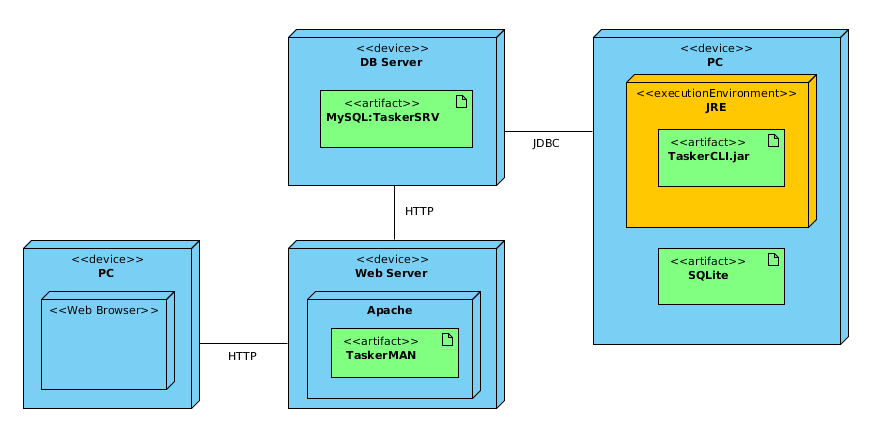
\includegraphics[width=\textwidth]{images/4.1/DeploymentDiagram} \\
The whole system will be composed of the following three components:
\begin{itemize}
	\item TaskerSRV (Database)
	\item TaskerMAN (Web Client)
	\item TaskerCLI (Desktop Client)
\end{itemize} 
TaskerSRV will be deployed onto a database server with a pre-installed MySQL
engine. It will store the critical data of the whole system and make it
accessible to both web and desktop clients through the specified protocols.
TaskerMAN will be deployed as a PHP web application onto an Apache web server
and it will be accessible from the Internet by any client with an installed web 
browser. Finally, TaskerCLI will be a desktop application written in Java, and it
will be deployed as a runnable jar onto a machine running the Java Runtime
Environment. Following the requirements specification\cite{se.qa.rs}, TaskerCLI will have to
operate both on-line and off-line. Therefore it will have a direct access to 
a local storage provided by the SQLite database.
\subsection{Applications interface}
Unlike the deployment diagram above, the component diagram below depicts the interaction of different modules or components of the proposed system. There are four major components that form the entire system. Only a black box view is shown here. This means that the components are not further decomposed to reveal the inner components. The opposite of this is a white box view which shows not only the major component but also the inner components that form the big picture. 
According to the design specification standard[1], only the simple black box view application interaction is relevant for now. A rundown of the actual interactions is as follows: \\
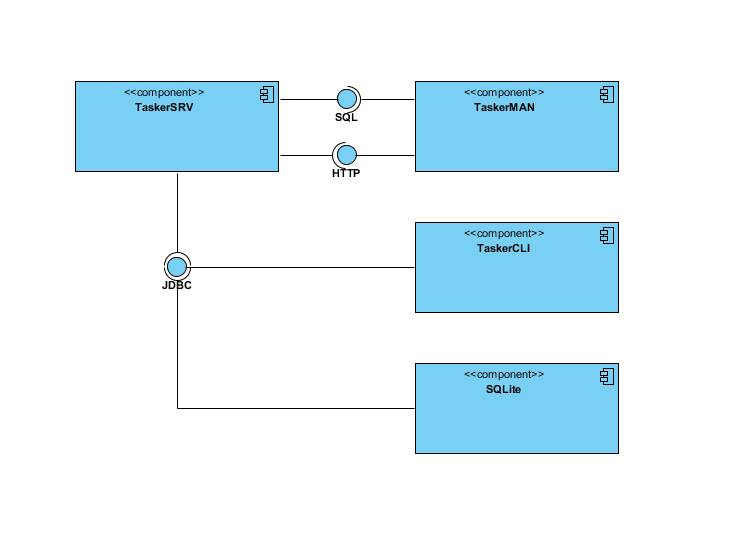
\includegraphics[width=\textwidth]{images/4.2/ApplicationsInterface} 
TaskerSRV - This component, representing the database, consists of one provided interface (solid circle) and two required interfaces (cup shaped). These are:
\begin{itemize}
	\item SQL(provided interface) : Provides an SQL interface, making it possible for the web application, TaskerMAN, to manipulate the database and carry the necessary operations outlined in the requirements[2] such as adding, editing, deleting users or tasks. 
	\item HTTP (required interface): Without the HTTP protocol the database would not be accessed by the TaskerMAN and no operation can take place.
	\item JDBC (required interface): The interface is required so that communication to the SQL can be established and give the required services to the client.
\end{itemize}
TaskerMAN - This component, representing the web application has one required interface (SQL) and one provided interface (HTTP). Without SQL provided by TaskerSRV, TaskerMAN will not be able to do anything. It will remain a useless dummy. Also if it can not provide the HTTP communication interface then it would not be able to access the database. \\
\newline 
TaskerCLI - This component representing the client has one provided interface (JDBC). Since it is using Java to connect to the database, TaskerSRV as well as SQLite will require that the interface JDBC be implemented on the client or else there will be no database connection. \\
\newline SQLite - This component representing the local database on the client has one required interface (JDBC) which makes it possible for the client to connect to it.
\section{INTERACTION DESIGN}
\subsection{Use-cases}
\subsubsection{TaskerMAN Use-Case}
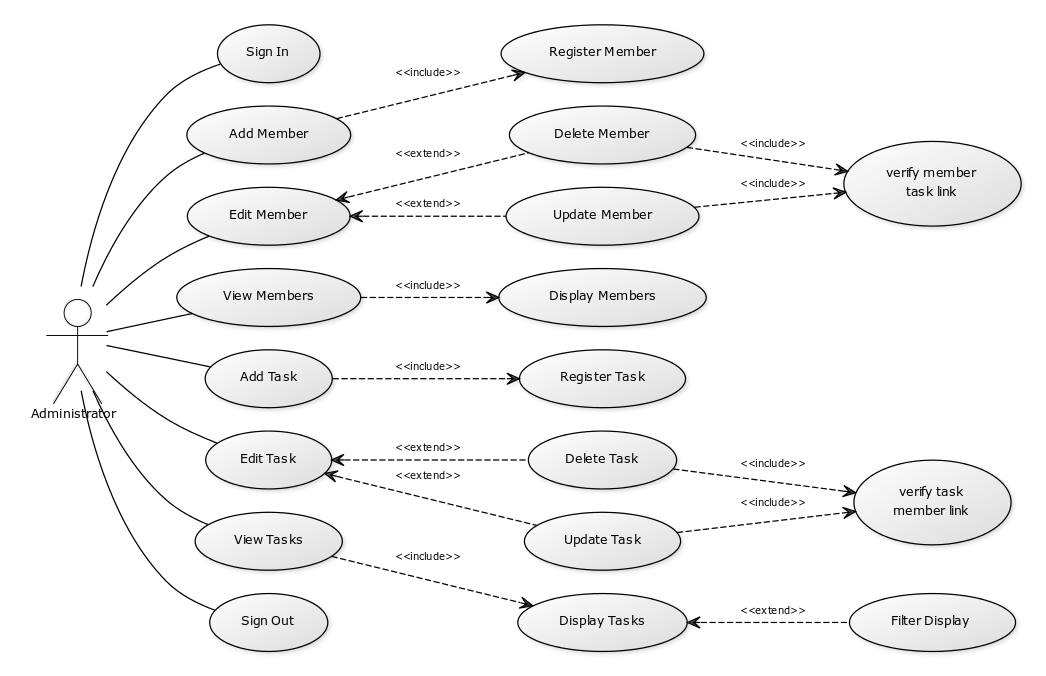
\includegraphics[width=\textwidth]{images/5.1/TaskerMANUseCase}
The TaskerMAN use case diagram above depicts clearly how the web administration application will be able to be used by the administrator.  The necessary functions depicted in the specification requirements\cite{se.qa.rs} are clearly accessible to the administrator after logging into the system. These functionalities are, add task, edit task, view tasks, filter display, add and edit member. The options update member and delete members as well as update task and delete task are labelled as extending.  This is because they are options and an administrator may or may not choose to delete a task or member.  Also they include a verification so that the administrator might be aware, for example, that a member to be deleted or updated might be currently assigned a task or vice versa.  Similarly the filter display is extended since an administrator may choose to filter display results or not.
Example usage scenario:
\begin{enumerate}
	\item The administrator logs onto the web application system.
	\item Selects "add member" and registers the members.
	\item Administrator clicks on "view members" to make sure the members are added.
	\item Administrator realises that a member name was misspelled. He or she clicks on "edit member" and selects the option "update member".  Necessary updates are done.
	\item Administrator then clicks on "add task" and a necessary form is displayed where data is entered.
	\item Administrator decides that the task was allocated to the wrong member.  He or she clicks on "edit task".  An appropriate page is loaded where the task can be selected and a reallocation can be carried out.
	\item Administrator decides that one more task is actually not needed.  He or she clicks on "edit task", selects the task and clicks on "delete task".  A prompt is displayed informing that the task is associated with a member.  If the administrator is comfortable to delete, then the action is executed.
	\item Administrator clicks on "view tasks" and all the tasks displayed.  An option is also available for the administrator to filter display results accordingly as specified in the requirements[8].
	\item The administrator has finished using the system and he or she clicks on "log out" and the session ends.
\end{enumerate}
\subsubsection{TaskerCLI Use-Case}
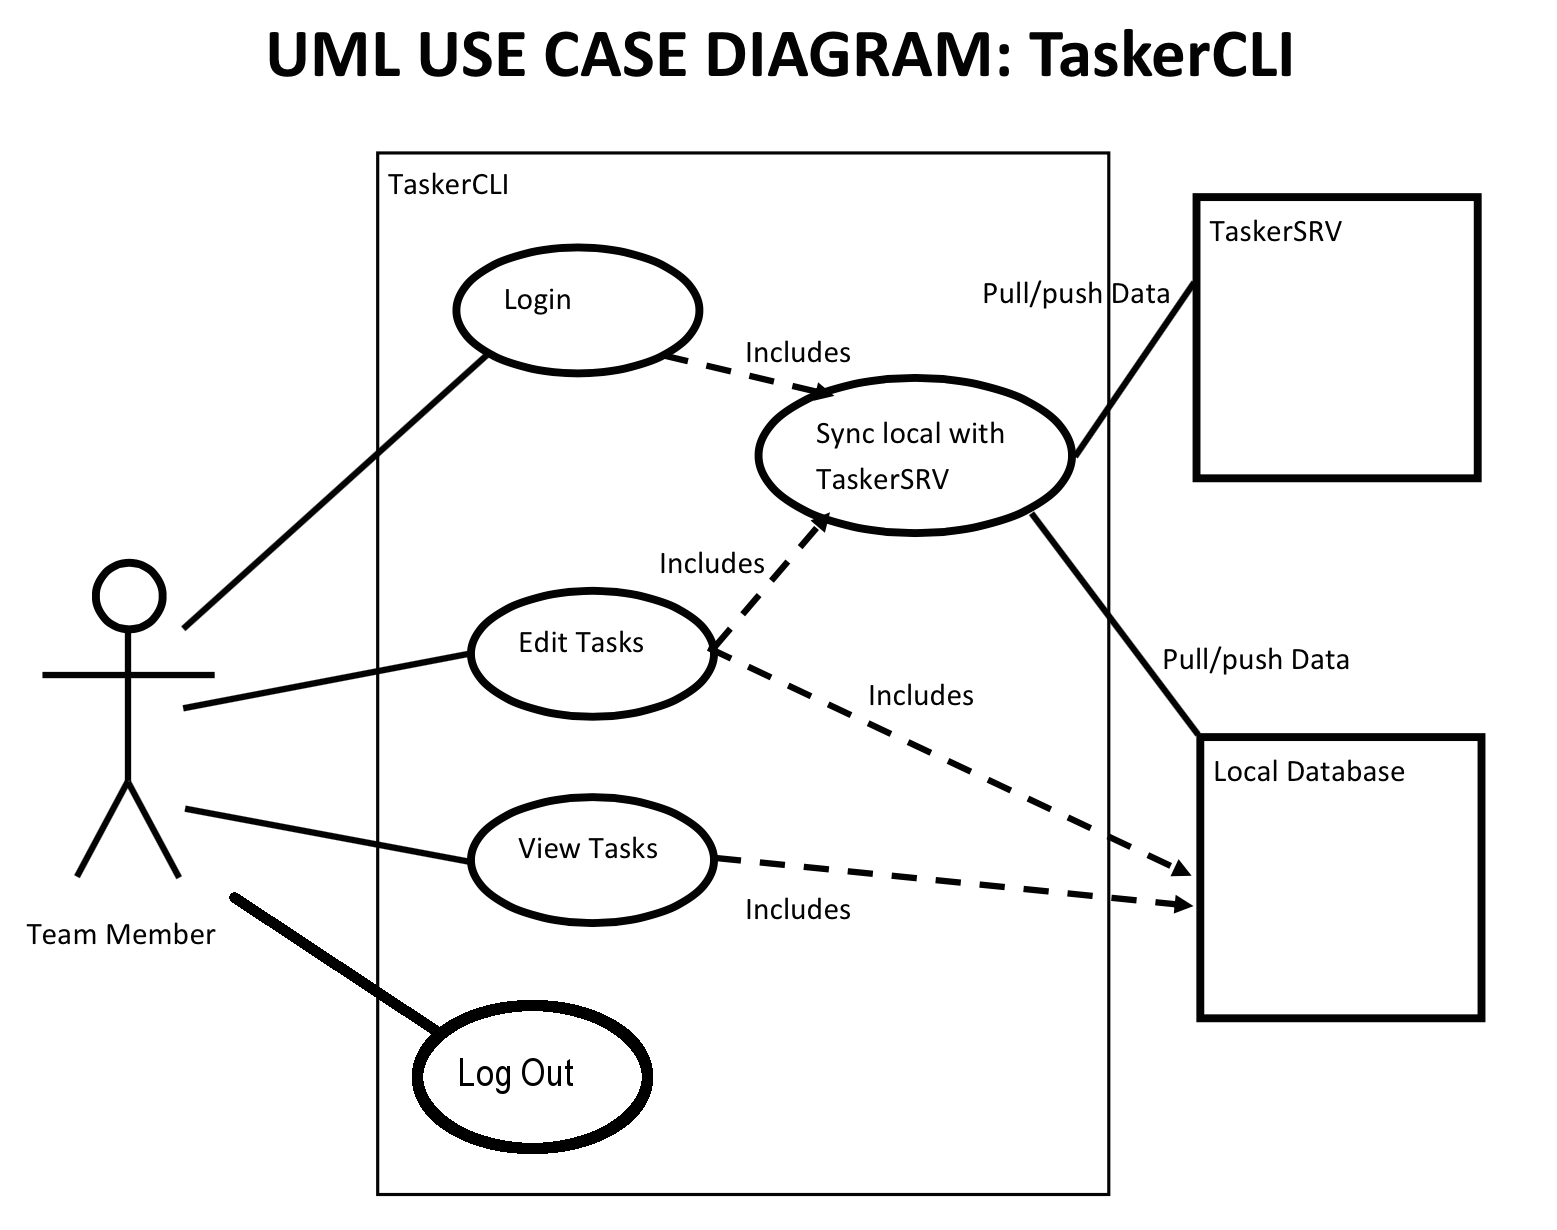
\includegraphics[width=\textwidth]{images/5.1/TaskerCLIUseCase}
The TaskerCLI use-case diagram above depicts how TaskerCLI will be used by "actors".  The diagram illustrates the different functions the application must contain as outlined in the requirements specification \cite{se.qa.rs}. These are user identification (login), local storage of tasks, task synchronisation and the function to edit tasks, both locally and to TaskerSRV. Example usage scenario:
\begin{enumerate}
	\item The actor logs onto the Java application.
	\item The application synchronises with TaskerSRV and pulls the tasks assigned to the actor and stores them to the SQLite database.
	\item The actor clicks on 'View Task' and the task information is loaded from the SQLite database and displayed on-screen.
	\item The actor confirms changes and clicks 'Edit Task', this will trigger another synchronisation to occur, and the changes will be pushed to TaskerSRV and to the SQLite database.
	\item The user has completed their actions and clicks 'Log Out', terminating the system.
\end {enumerate}	
\subsection{User Interface design}
\subsubsection{TaskerMAN Interface Design} 
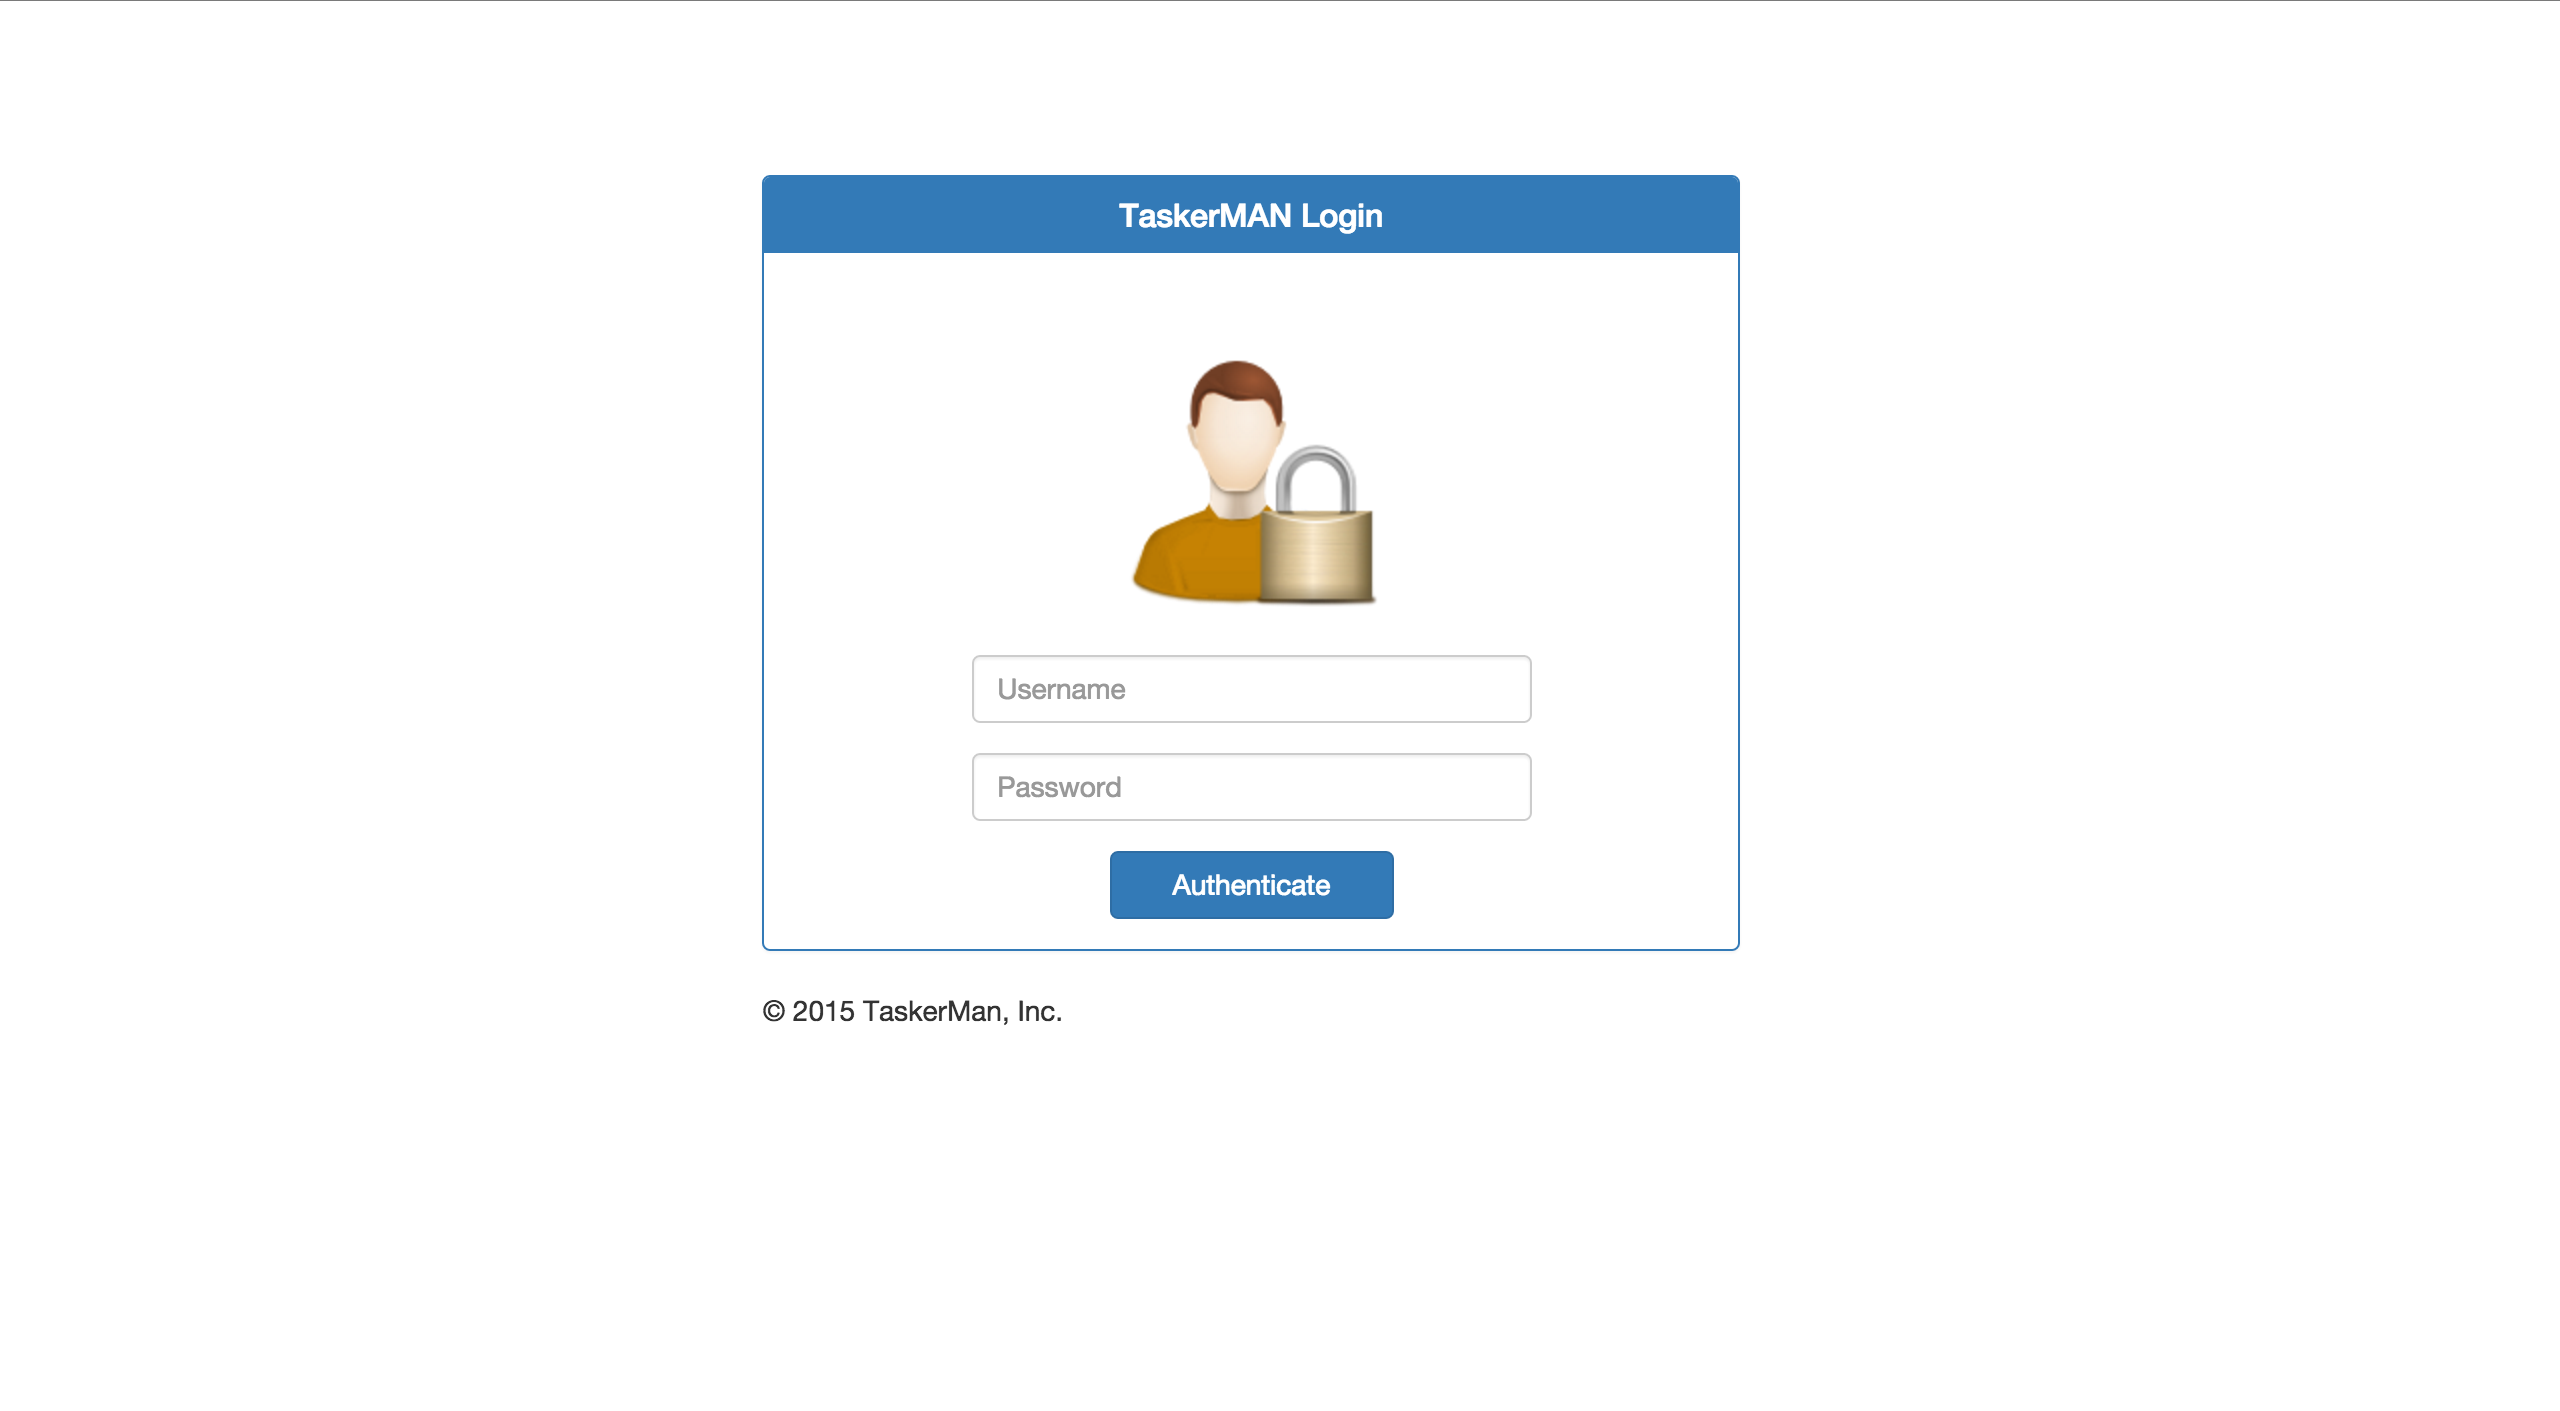
\includegraphics[width=0.75\textwidth, center]{images/5.2/TaskerMANAuthentication} \\
This is the authentication page of our website with the address `/taskerMAN/login.php'. Upon attempting to enter any page of the website, should a local session not exist users will be redirected to this page where they will be required to enter their login credentials. If the credentials entered are incorrect then the screen will simply refresh, and the fields will appear blank again. If the credentials are correct then the user will be redirected to the home page of the website. If at any point in the user's session they click the logout icon in the top right of any of the website's pages, the session will be destroyed and they will be redirected back to this authentication page.\\~\\
\newline
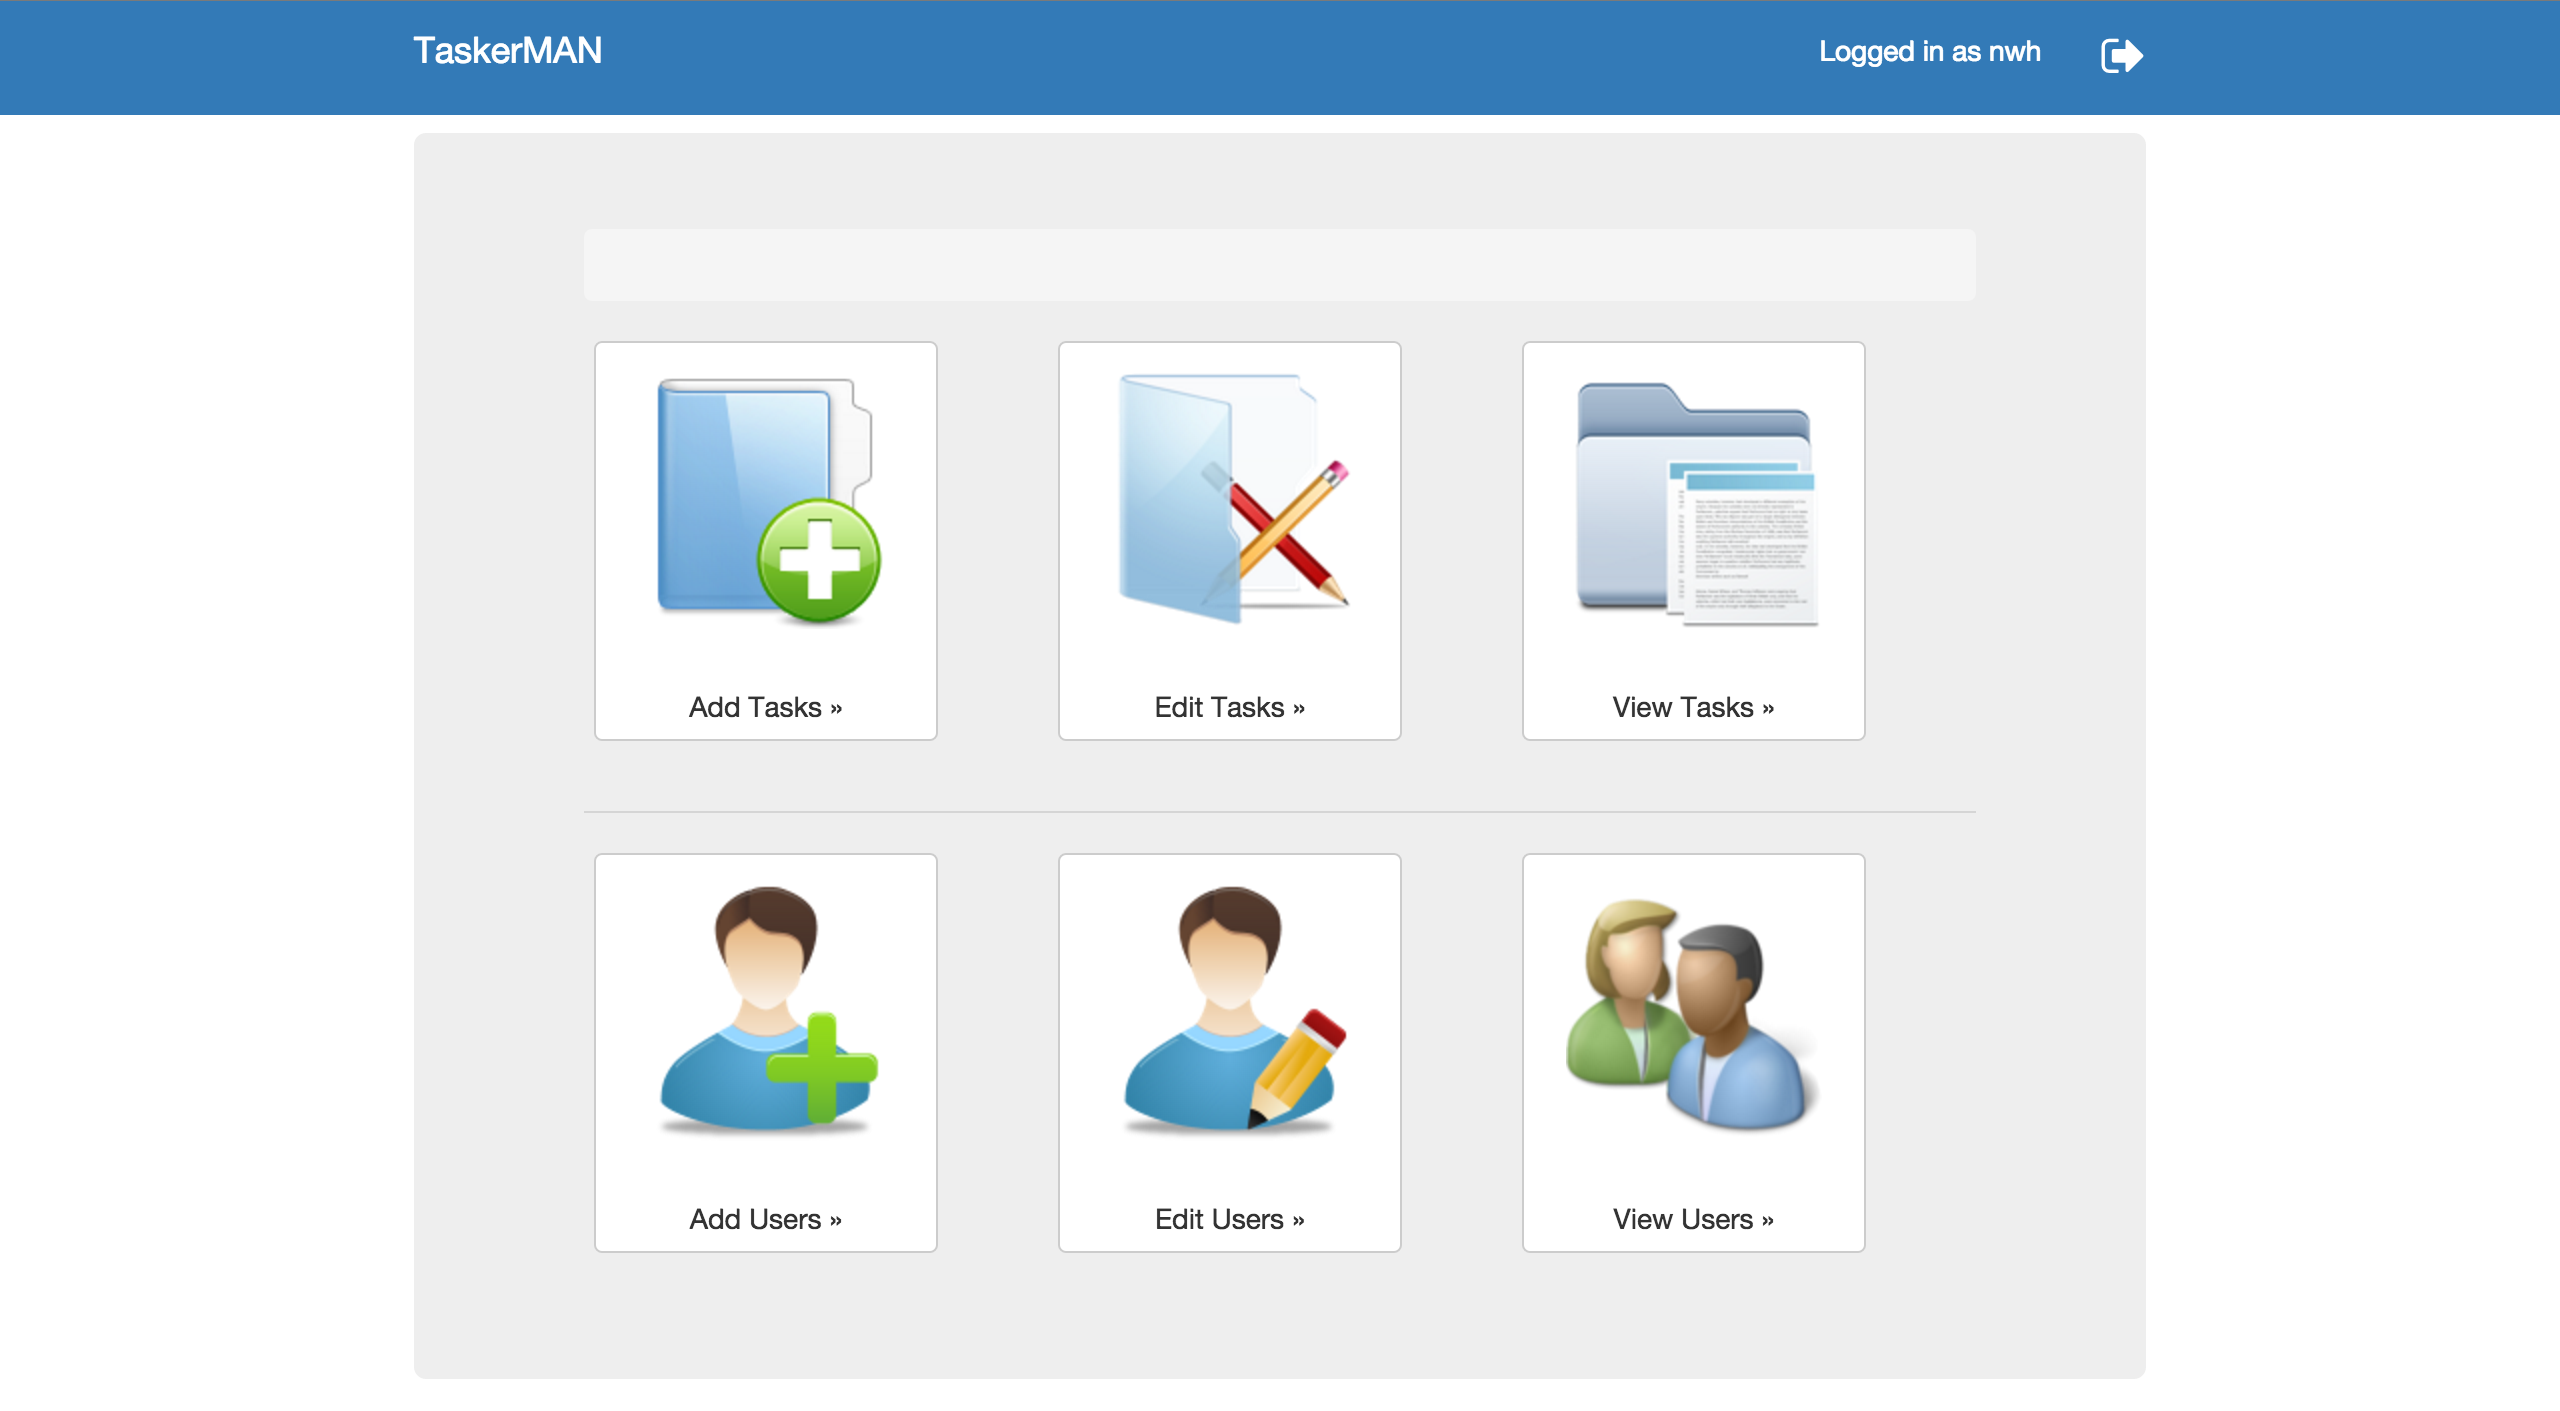
\includegraphics[width=0.75\textwidth, center]{images/5.2/TaskerMANHomePage} \\
This is the home page of the web interface with the address `/taskerMAN/index.php', it is very easy to use and presents you with six options which provides very quick access to all aspects of the Tasker. To begin we will click on the `Add Users' button. This will re-direct us to the `Add User' page. \\~\\
\newline
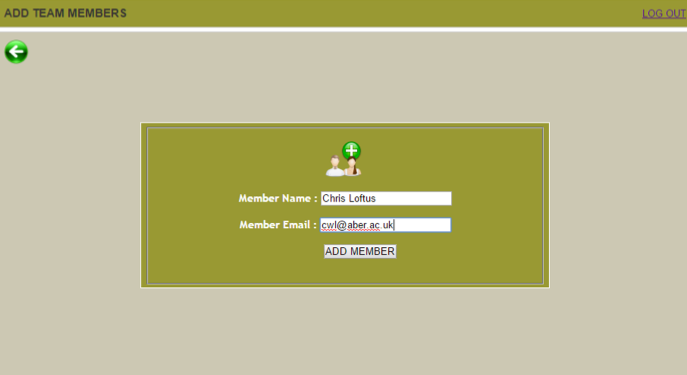
\includegraphics[width=0.75\textwidth, center]{images/5.2/TaskerMANAddUser} \\
Here within the `Add User' page with the address `/taskerMAN/adduser.php', you will be presented with the form above which enables you to create a user by submitting their name, e-mail and password. Upon pressing the `Add User' button the new member will be added to the database as required \cite{se.qa.rs}. Clicking on the `backwards arrow' in the top-left corner allows users to return to the home page. In fact the `backwards arrow' exists within all of the sites internal pages, and has the same function as clicking on the `TaskerMAN' logo in the top-left corner which is to return to the website's home page.\\~\\
\newline
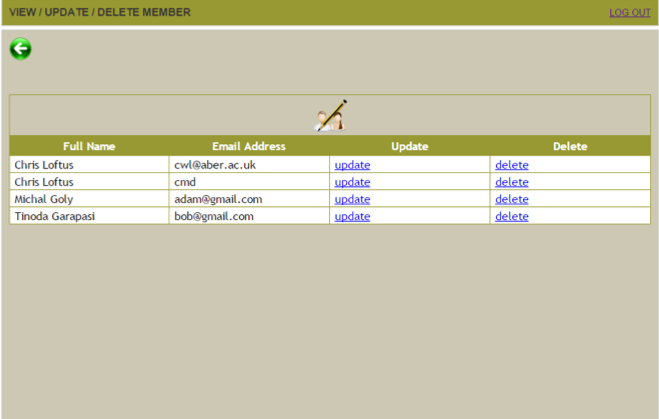
\includegraphics[width=0.75\textwidth, center]{images/5.2/TaskerMANEditUser} \\
To update or delete user data as required \cite{se.qa.rs} click on the `Edit Users' button from the home page and you will be presented with this page with the address `/taskerMAN/editusers.php', displaying user's names, e-mail addresses and options to update/delete their information, clicking on the `update' icon of a user re-directs to a page with the address `/taskerMAN/updateusers.php' which has the same interface as the 'Add Users' page where name and password can be updated, clicking on the `delete' icon will prompt the user to verify their action with an `Are you sure you want to delete this user?' message with buttons for `yes' and `no'. Clicking on `no' will redirect the user back to `Edit Users' portal, clicking on `yes' will cause a delete command to be submitted to the database to remove the user from the database, a message displaying this action will be displayed on screen. \\~\\
\newline
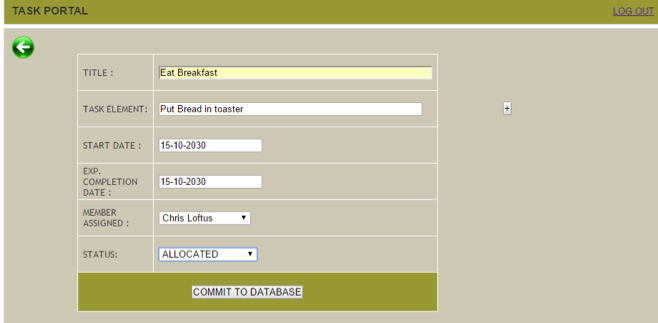
\includegraphics[width=0.75\textwidth, center]{images/5.2/TaskerMANAddTask} \\
Clicking 'Add Tasks' from the home page will re-direct to the task portal with the address `/taskerMAN/AddTaskBoot.php'. This is where users can make tasks which will then be allocated to members in the remote database as required \cite{se.qa.rs}. This task portal layout will also be used when updating tasks, the only difference being that when updating a task there will be an option for the user to set a task as `Abandoned' as required \cite{se.qa.rs}. `Task Title' and `Task Element' will be text fields for user input, whereby clicking on the `+' icon will cause another `Task element' field to continuously drop below the previous field. The field where you specify which user the task will be allocated to is a drop down field containing all of the members currently present in the remote database.` Start Date' and `End Date' are drop down calendars created with JavaScript, this allows us to make it impossible to allow users to set an end date which is before the start date. The `Add Task' button then adds the task to the database and will then sync up with the client, a confirmation screen is then shown to show the user that the task has been successfully added. \\~\\
\newline
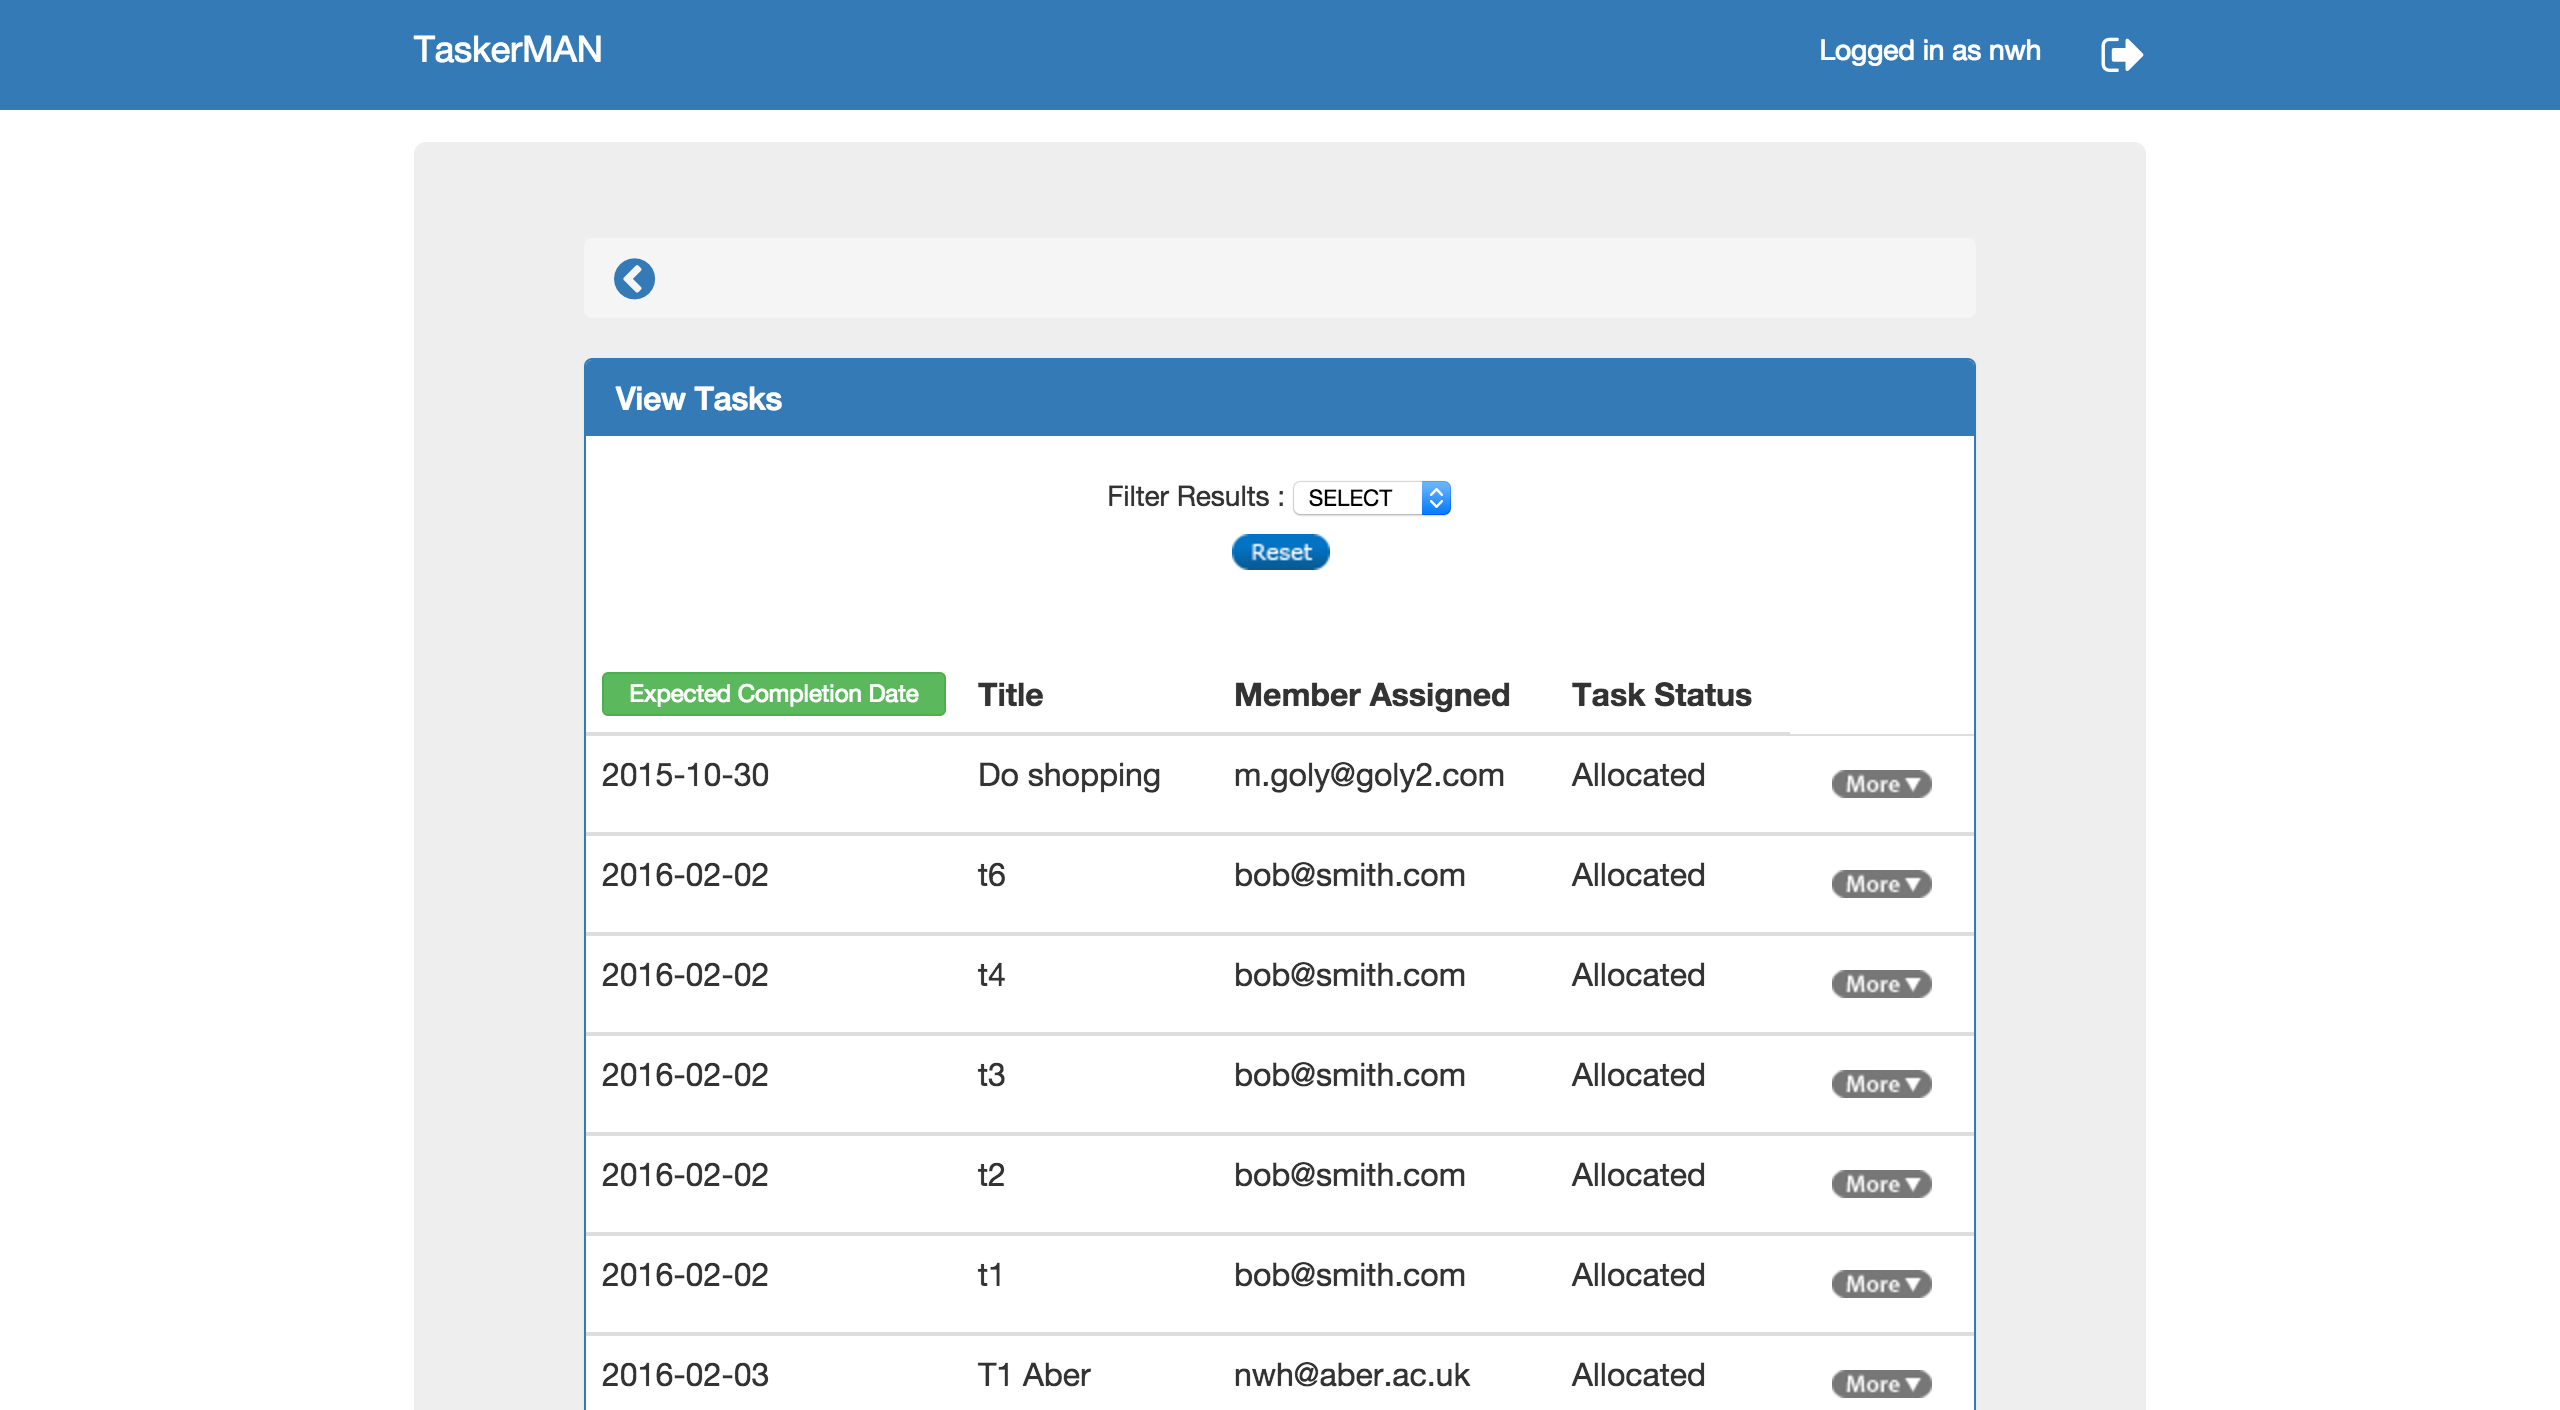
\includegraphics[width=0.75\textwidth, center]{images/5.2/TaskerMANViewTask} \\
Clicking `View Tasks' from the home page will redirect to this page with the address `/taskerMAN/viewtasks.php'. Here you can view all the tasks, as well as their title, expected completion date, member assigned to and task status. By default the tasks are sorted by expected completion date as required \cite{se.qa.rs}, with the most impending tasks displaying at the top. This can be changed however by clicking the drop down list to filter the results, either by member assigned to or by task status. To view the task elements related to a task you click on the `More' button of a task.  \\~\\
\newline
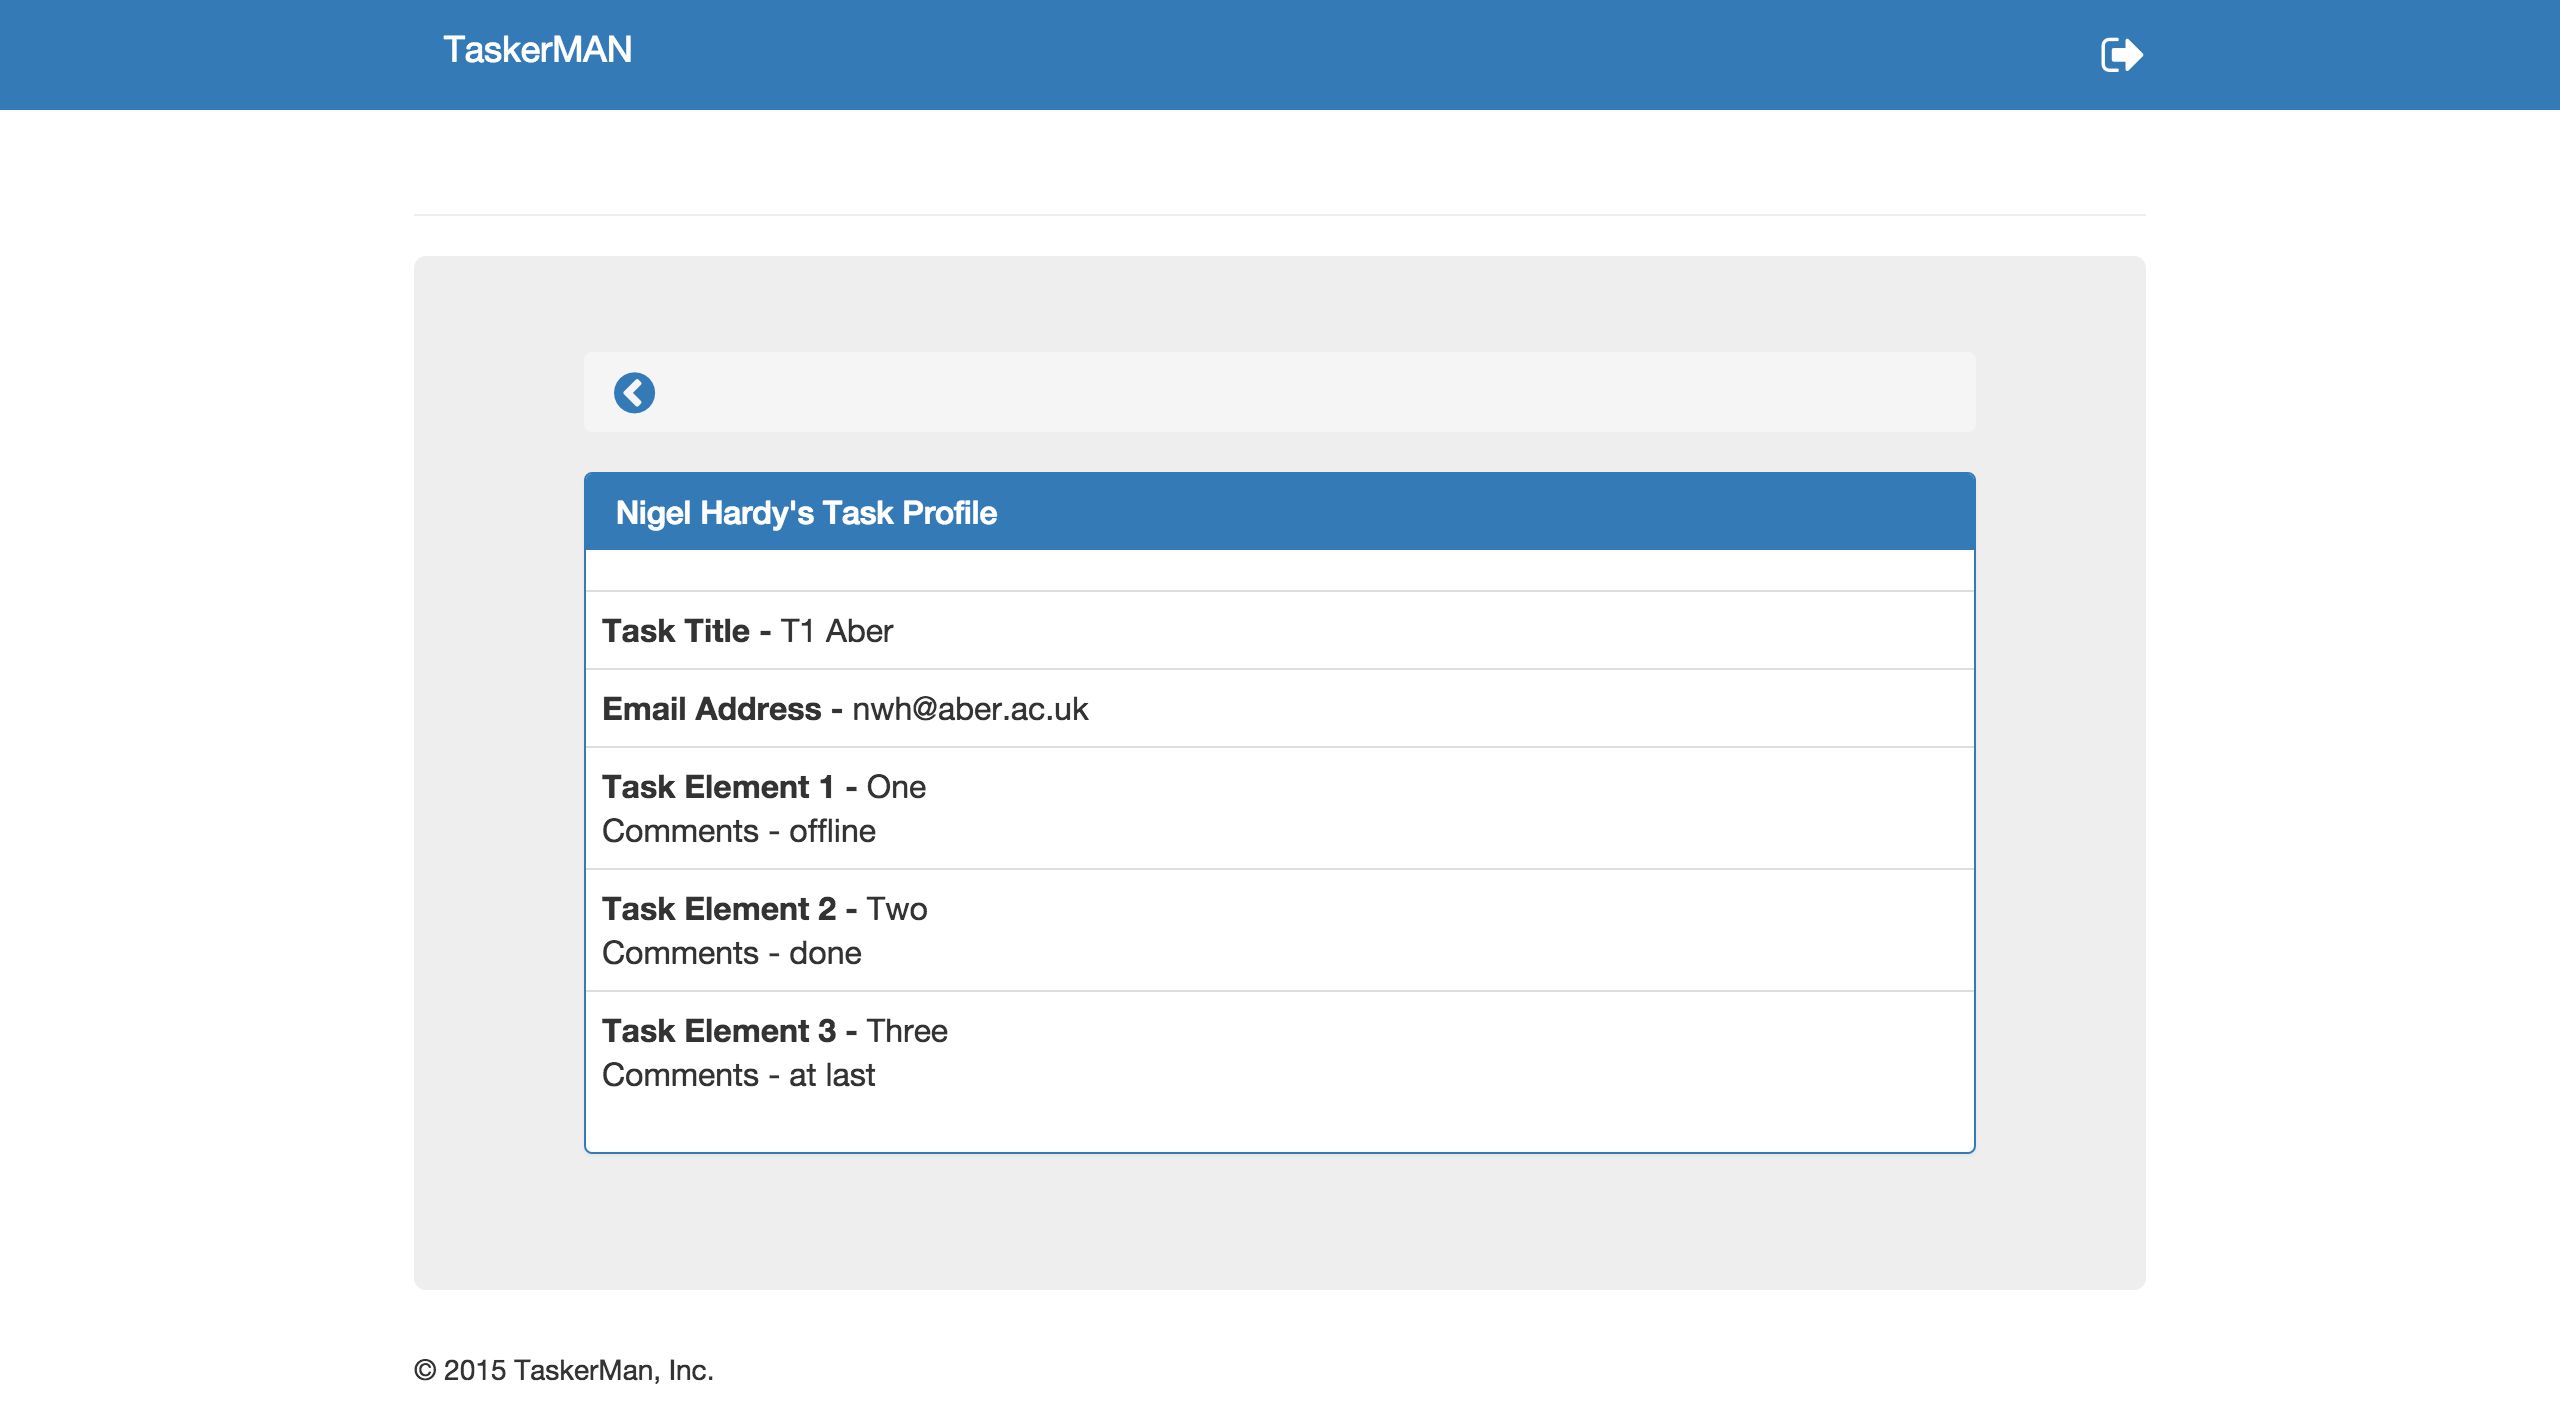
\includegraphics[width=0.75\textwidth, center]{images/5.2/TaskerMANViewTask2} \\
Here is the display of clicking on the `More' button of a particular task. This view allows the user to view a task, the user assigned to the task, the task elements associated with the task, as well as comments made about the task elements from the TaskerCLI application as required \cite{se.qa.rs}. The task elements and comments are fetched from the remote database. \\~\\
\newline
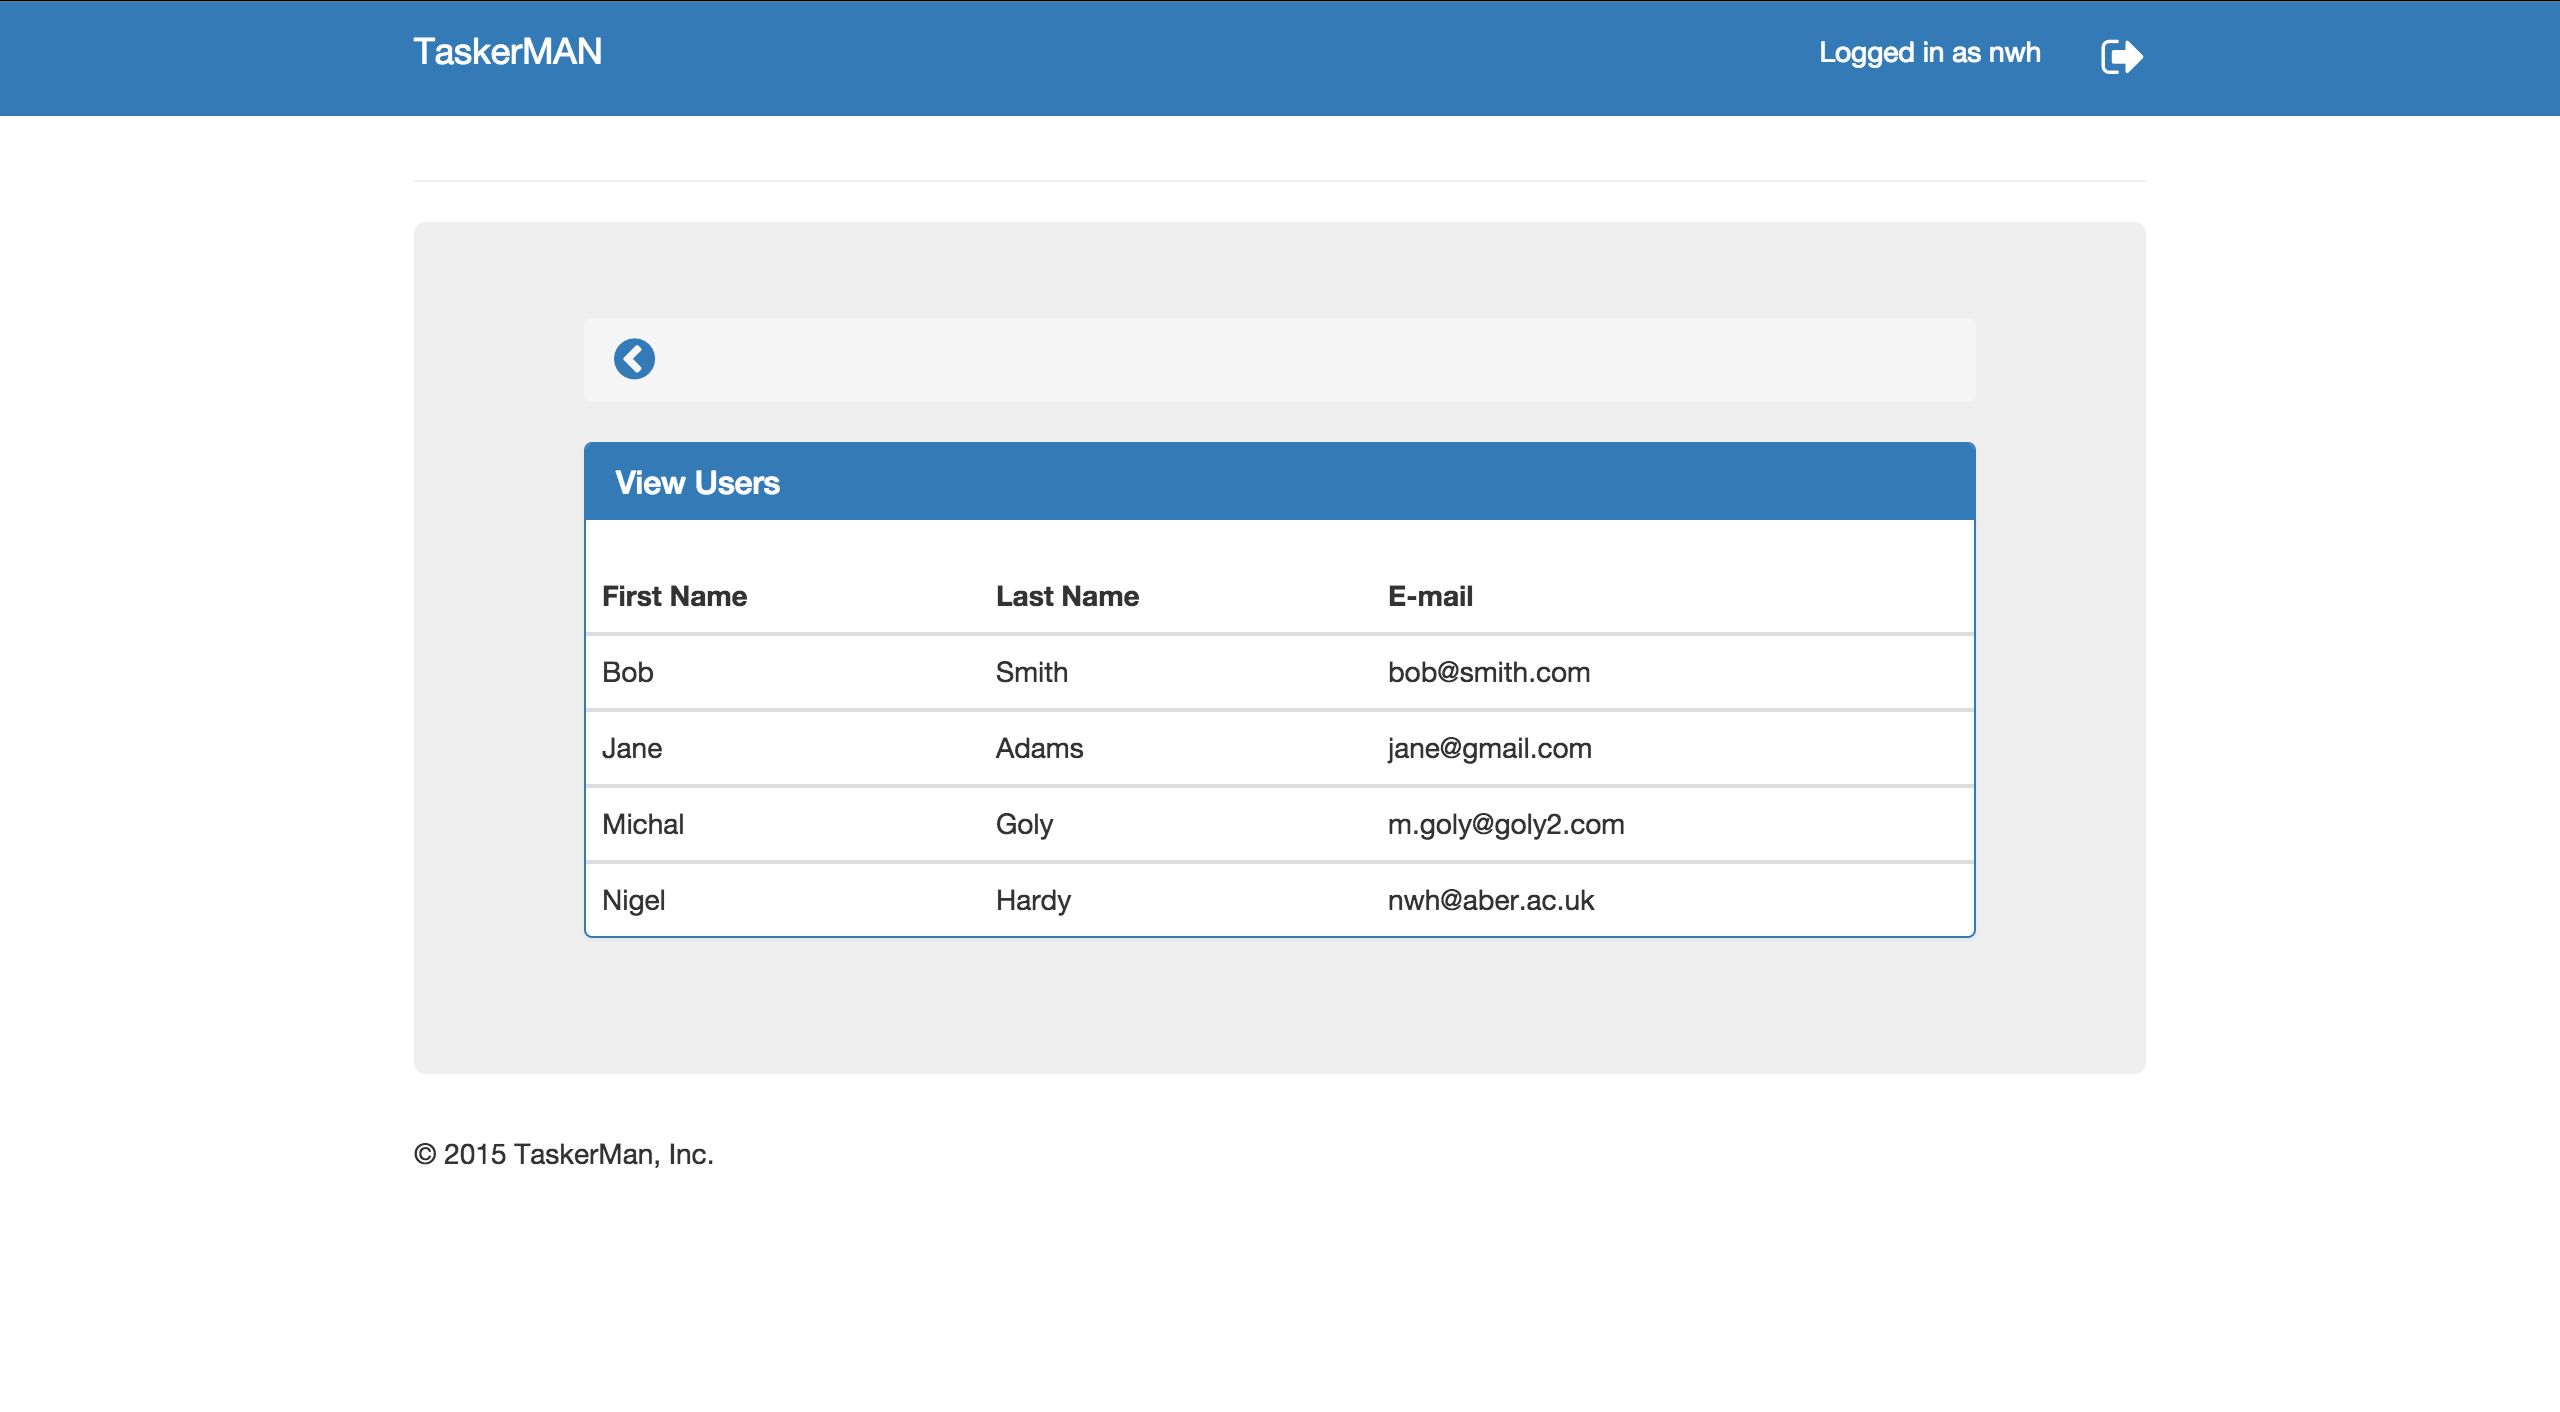
\includegraphics[width=0.75\textwidth, center]{images/5.2/TaskerMANViewUsers} \\
From the home page of the website clicking on `View Users' will display the view users page with the address `/taskerMAN/viewusers.php'. This page simply fetches all the users currently present in the remote database and displays them on screen with their first name, last name and e-mail. \\~\\
\newline
\clearpage

\subsubsection{TaskerCLI Interface Design} 
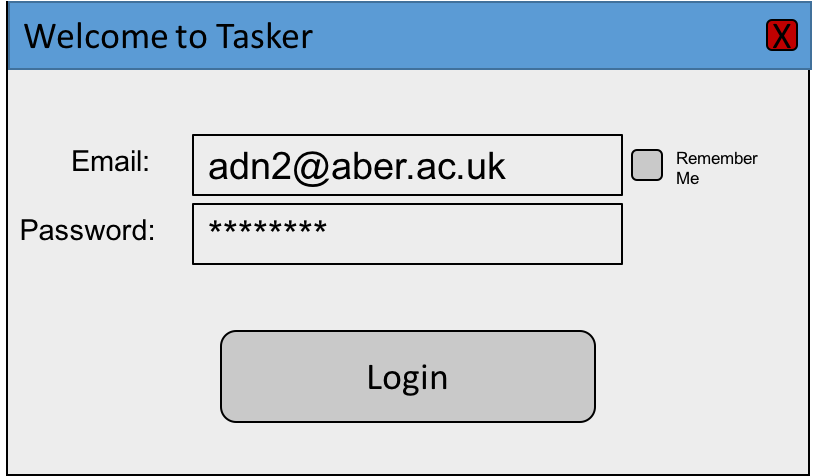
\includegraphics[width=0.5\textwidth, center]{images/5.2/TaskerCLILogin} \\
The login screen, the first screen to appear when the client loads. TaskerCLI does not synchronise with the database until the user has logged in as specified in Requirements Specifications.\cite{se.qa.rs} \\~\\
\newline
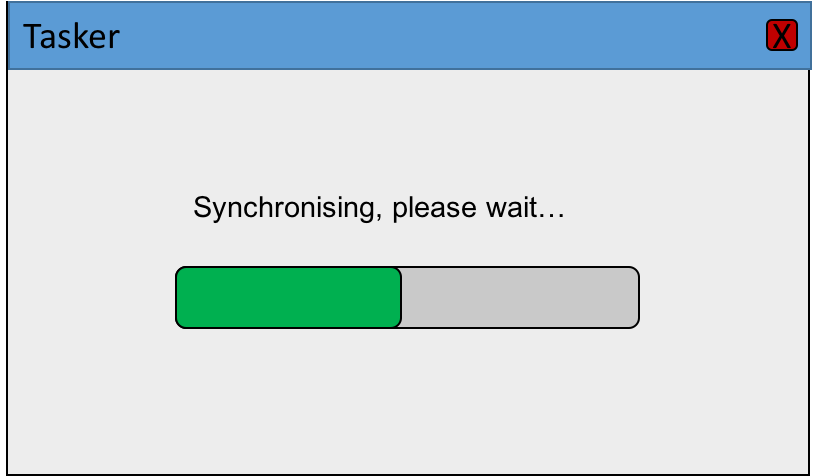
\includegraphics[width=0.5\textwidth, center]{images/5.2/TaskerCLILoading} \\
The synchronisation screen occurs between the login and main client page. As per the requirements specifications \cite{se.qa.rs} this screen will also occur before and after local editing if network access is available, as well as occurring every 5 minutes by default should no local editing take place. This will display the relevant information from the database as it's downloading the data. Ideally this will be a fast enough task that this screen should be seen for as little time as possible. \\~\\
\newline
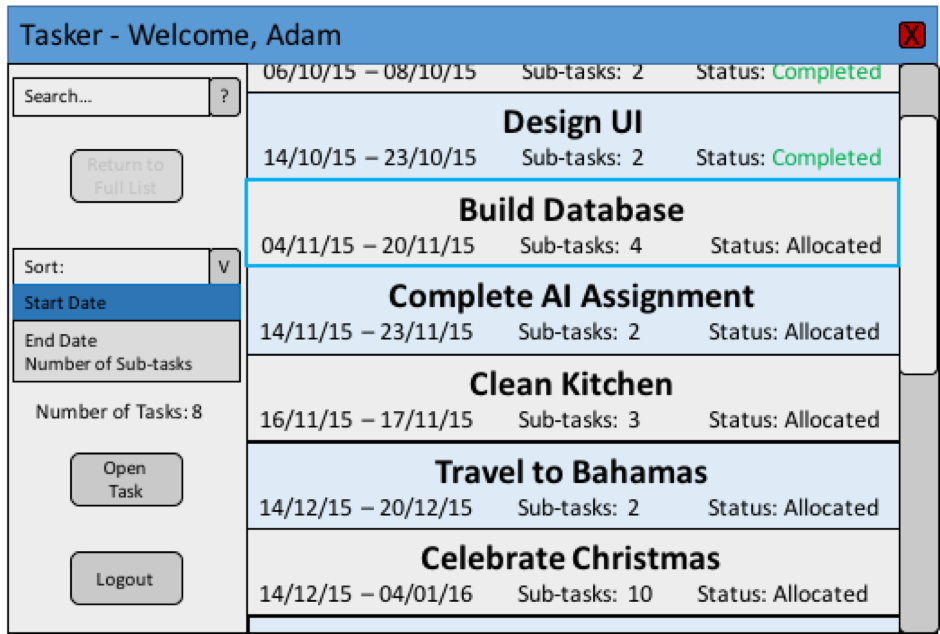
\includegraphics[width=0.75\textwidth, center]{images/5.2/TaskerCLIMainScreen} \\
The 'Main Screen' of TaskerCLI. It shows a list of tasks assigned to the person who signed in, as well as options for sorting and searching through the list. Clicking on the 'Log Out' button will re-direct the user back to the login authentication screen. Double clicking a task's panel, or selecting a task and clicking the 'open task' button shows more detail about the task \cite{se.qa.rs}, as well as the editable parts, such as the completed/allocated attribute and the sub-task list comments. In this example we'll double-click on the "Build Database" task. \\~\\
\newline
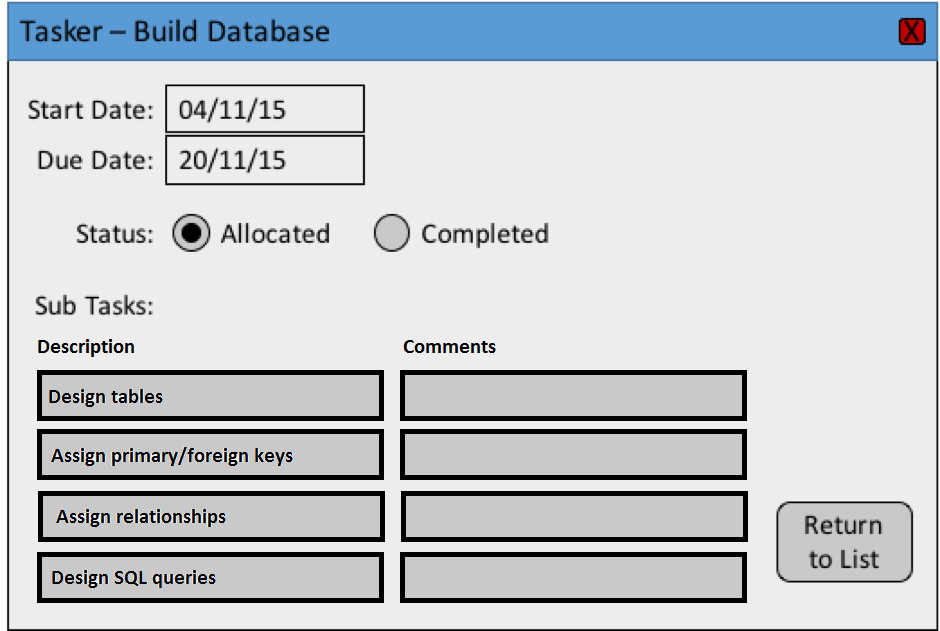
\includegraphics[width=0.75\textwidth, center]{images/5.2/TaskerCLITaskInfo} \\
This screen shows more details about the "Build Database". It displays all the task's information and allows the user to edit task step comments and change task's status \cite{se.qa.rs}. \\~\\
\newline
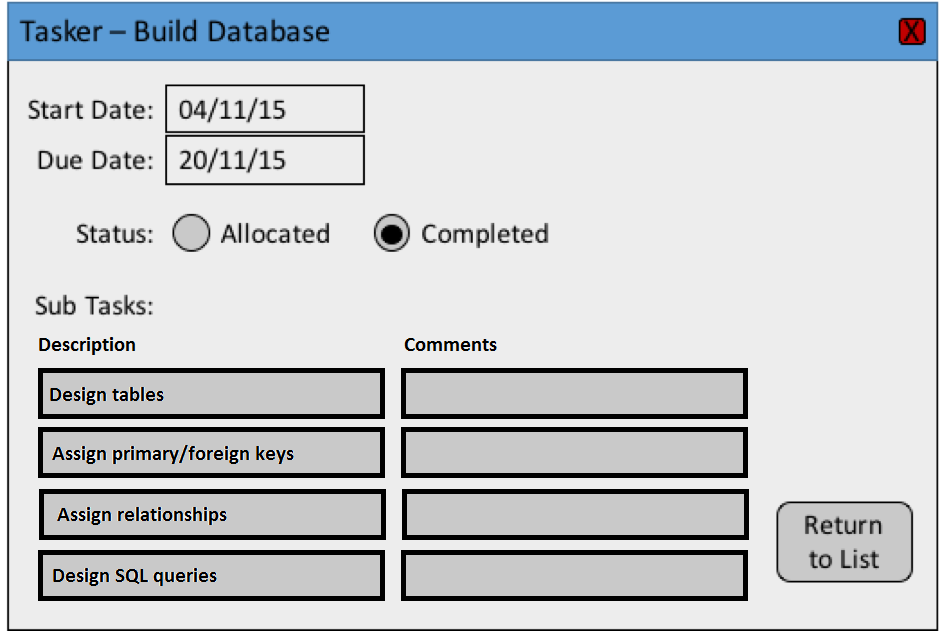
\includegraphics[width=0.75\textwidth, center]{images/5.2/TaskerCLITaskUpdated} \\
In this image we've changed the status to 'Completed'. We can press the 'Return to List' button to return to the 'Main Screen'. Doing so will prompt the synchronisation screen to appear and an attempt will be made to connect to the network and update the information on the remote MySQL database. If unsuccessful the user will still be re-directed back to the 'Main Screen', however the client will be now operating locally using the local SQLite database until a connection with the MySQL can be re-established.\\~\\
\newline
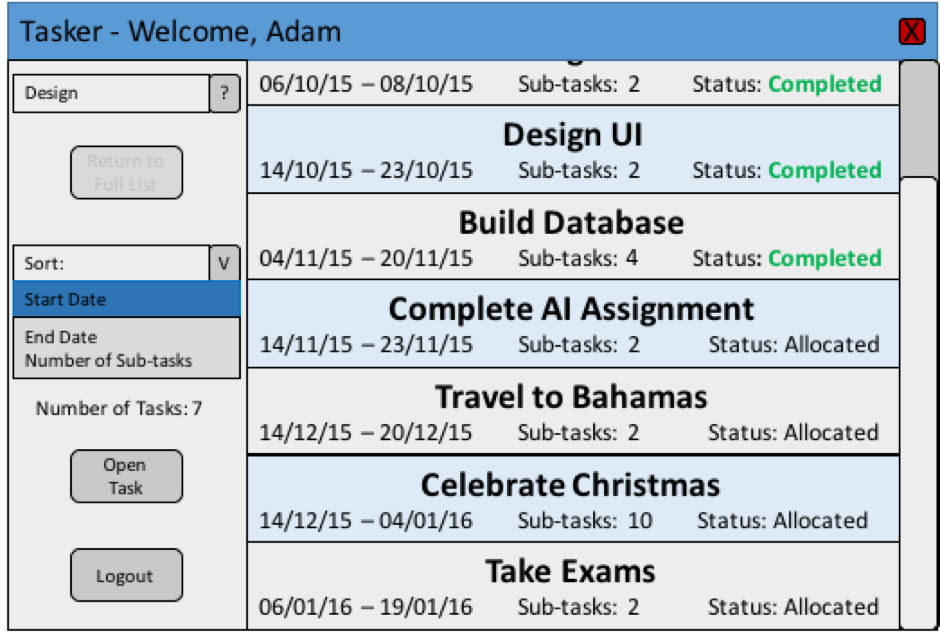
\includegraphics[width=0.75\textwidth, center]{images/5.2/TaskerCLIMainScreenUpdated} \\
Note the changes made are now reflected in this list. Also note that the task named 'Clean Kitchen' has disappeared. This is something that could happen if said task were marked 'Abandoned' via TaskerMAN while the user was editing a task within TaskerCLI, provided there is a network connection. \\~\\
\newline
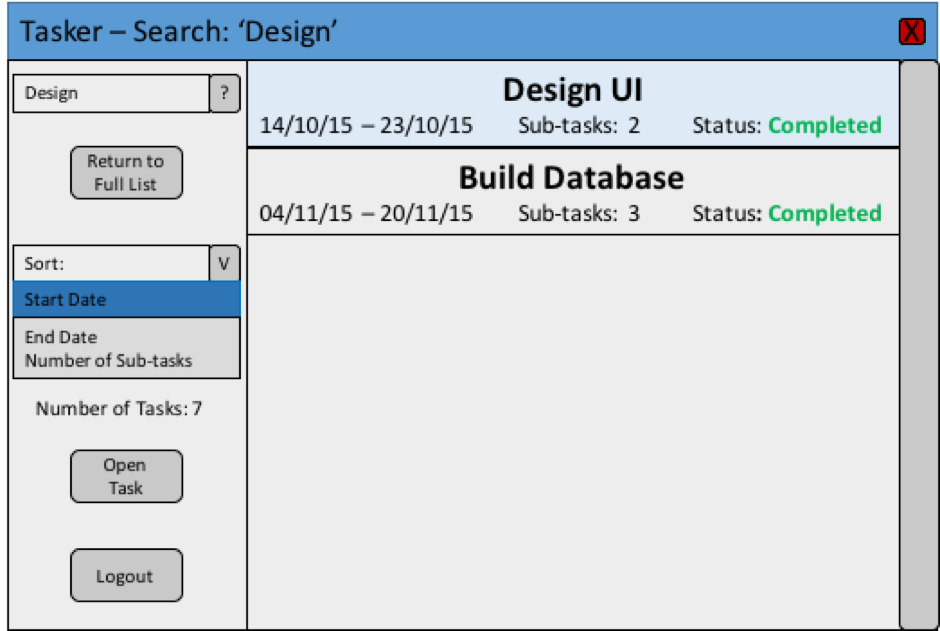
\includegraphics[width=0.75\textwidth, center]{images/5.2/TaskerCLIMainScreenSearch} \\
Searching using the text box searches for the string provided in the task's name, and/or it's sub-tasks. Also note that the 'return to full list' button is only selectable if there is currently a search parameter in the search box.\\~\\
\newline
There is a large focus on designing the interfaces of both TaskerCLI and TaskerMAN to be intuitive to regular computer users \cite{se.qa.rs}.
\clearpage
\section{Component Description}
\subsection{TaskerMAN Component Description}
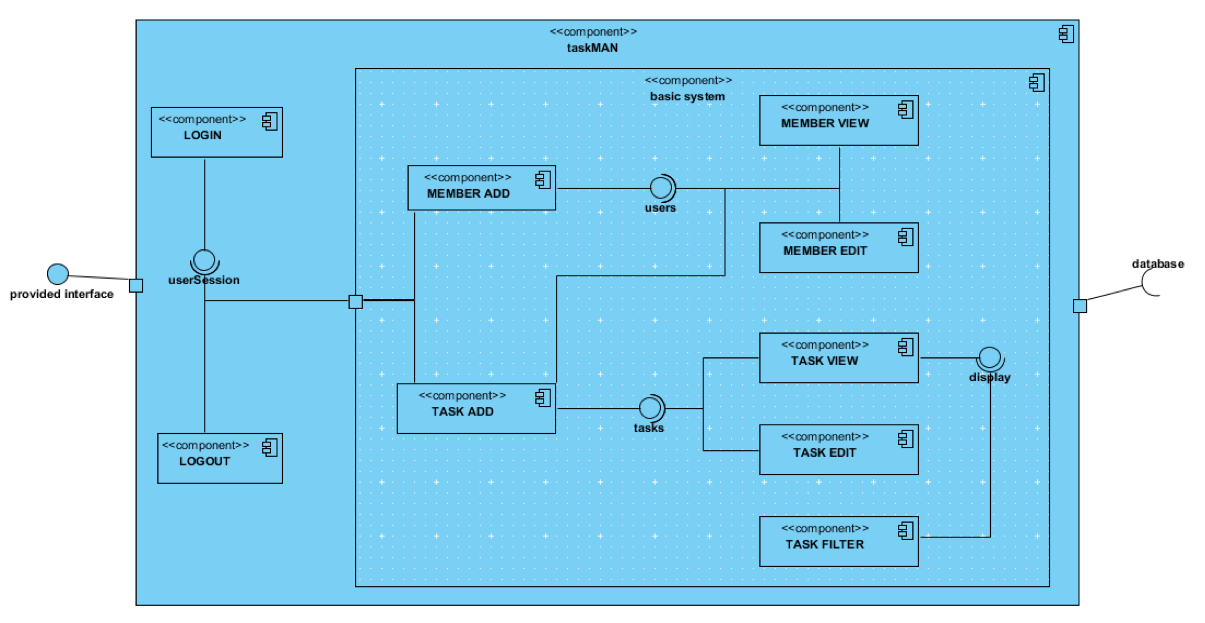
\includegraphics[width=1\textwidth, center]{images/Detailed-Design/TaskerMANComponentDiagram}
The component diagram above shows a further and advanced decomposed version unlike the previous diagram submitted before.  As can be seen, two external interfaces are provided with one connecting to the database and the initial user interface which through a given port lets us use the login component which gives access to the basic system.  The first point to using the basic system is either through member add or task add as shown. These two sub components provide respective interfaces to other sub components.  For example its clear that the TASK\textunderscore ADD component requires  an interface from MEMBER\textunderscore ADD, at the same time it also provides an interface which is then used by TASK\textunderscore VIEW and TASK\textunderscore EDIT component. TASK\textunderscore VIEW sub component also provides an interface which is then used by the TASK\textunderscore FILTER sub component. 
The LOGOUT sub component is shown as requiring a session established after the LOGIN component has been initiated. 
\clearpage
\section{Significant Classes} 
\subsection{TaskerCLI Significant Classes}
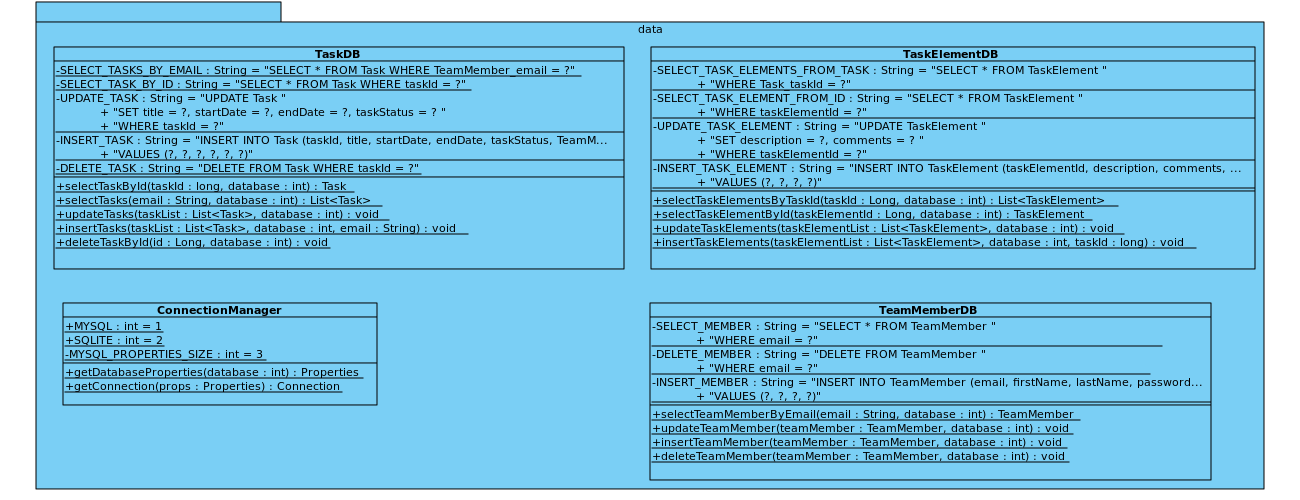
\includegraphics[width=\textwidth]{images/Detailed-Design/taskerCLI_design1.png}

  We are using the Data Access Object design pattern, to abstract our database contents and more easily access it from within the Java client.
  We have abstracted our database tables into Java entities, as an example, in the image below TaskElement class corresponds to the 
  TaskElement table in the databases.
  In order to access the abstracted data from the database we use a selection of data access classes (see below).
  These classes apply the DAO pattern, and call methods in order to send properly formatted SQL queries to the appropriate database, and present the result of the queries in the form of the previously described entities. 
  This object is then used by the UI classes in order to generate the view.
  
  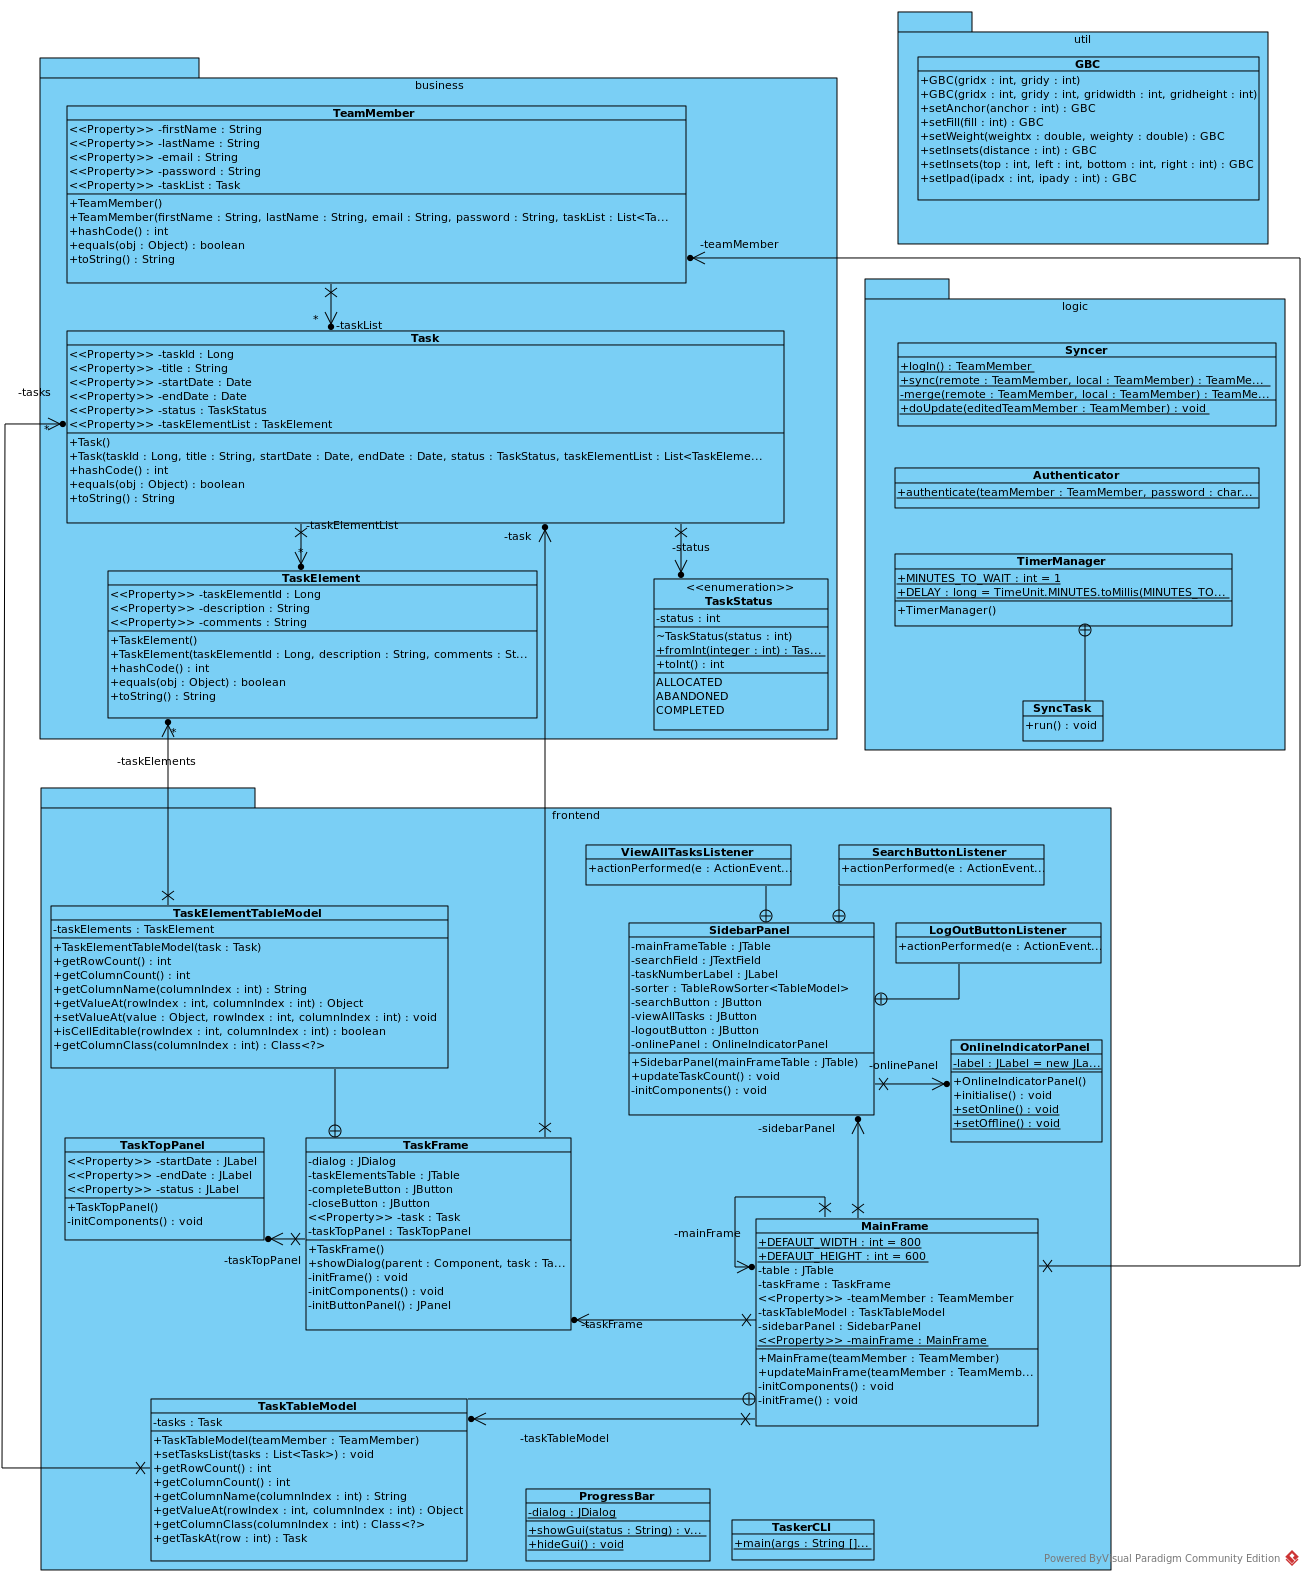
\includegraphics[width=\textwidth]{images/Detailed-Design/taskerCLI_design2.png}

  \subsubsection{Description of each significant Class}

  \begin{itemize}
  		\item \textbf{TeamMember} class abstracts the TeamMember table in both databases. Its instance variables correspond to columns inside 
  		databases and can be accessed and modified using the getters and setters provided. Instance of this class will be used to populate
  		the user interface with data in the program.
  		\item \textbf{Task} class abstracts the Task table in both databases. Its instance variables correspond to columns inside 
  		databases and can be accessed and modified using the getters and setters provided. Each task has an associated list of task elements. The status of a task is stored as an integer in the database and is then transformed to an appropriate \textbf{TaskStatus} Enum inside the program.
  		\item \textbf{TaskElement} class abstracts the TaskElement table in both databases. Its instance variables correspond to columns inside 
  		databases and can be accessed and modified using the getters and setters provided. 
  		\item \textbf{TeamMemberDB} class is one of the data access classes in the DAO pattern. It provides useful methods which can be used to retrieve and update the \textbf{TeamMember} objects in both databases. For example the \texttt{selectTeamMemberByEmail} method will as expected acquire the connection to either the MySQL or SQLite database, prepare a suitable query statement, construct the \textbf{TeamMember}
  		object and return it back to the caller. This is a really powerful concept which abstracts the raw SQL from the graphical user interface. After we make some changes to the object, we can use a single method \texttt{updateTeamMember} to put it back to the database. 
  		\item \textbf{TaskDB} class is very similliar to the previously described \textbf{TeamMemberDB} class. It also is a part of the DAO pattern and provides direct access to the information stored in the task table in both databases. It will be typically only used by the previosuly mentioned \textbf{TeamMemberDB} to construct the complete \textbf{TeamMember} object.
  		\item \textbf{TaskElementDB} class is basically the same as the previous one, but it enables the access to the TaskElement table in both databases.
  		\item \textbf{ConnectionManager} class can be used to actually connect to both databases. It enables the caller to acquire a \texttt{Connection} object to either the remote MySQL (TaskerSRV), or locally run SQLite. \textbf{ConnectionManager} is capable of registering appropriate JDBC drivers depending on the connection required. 
        \item \textbf{Syncer} class contains the logic for conflict resolution between the contents of the two databases within its \texttt{merge} method. The merge method takes two \textbf{TeamMember} objects, generates a canonical TeamMember object, which is supplied to the databases and UI; the merge method is called via the \textbf{sync} method, which loads the \textbf{progressBar}, and sets the status of the \textbf{onlineIndicator}. The Syncer class also contains the \texttt{login} method, displaying a dialog for user login, authenticaring using the \textbf{Authenticator} class and returning an appropriate \textbf{TeamMember} object.
        \item \textbf{TimerManager} Class used to invoke \textbf{sync} at regular intervals.
        \item \textbf{Authenticator}  provides a static method to provide functionality to the \textbf{login} method to check passwords. Using BCrypt the passwords are hashed to keep them secure, and are encrypted in the databases. 
        \item \textbf{TaskerCLI} class is the main class that is run when the application begins. It calls the \textbf{Syncer} classes \texttt{login} method and passes the returned \textbf{TeamMember} onto the UI Classes.
        \item \textbf{MainFrame} extends \textbf{JFrame} class is the primary view after the login menu, and displays a \textbf{TeamMember} object's Tasks in a sortable JTable, clicking on this invokes \textbf{TaskFrame}. Also displays \textbf{SidebarPanel}.
        \item \textbf{SidebarPanel} extends \textbf{JFrame} class is used for controls within \textbf{SidebarPanel}, such as logging out and searching tasks.
        \item \textbf{TaskFrame} extends \textbf{JDialog} class is used to display details of a task when invoked by \textbf{MainFrame}. Allows editing of \textbf{TaskElement} and also marking of a Task as complete.
  \end{itemize}
\clearpage  
  
\subsection{TaskerMAN Significant Classes}
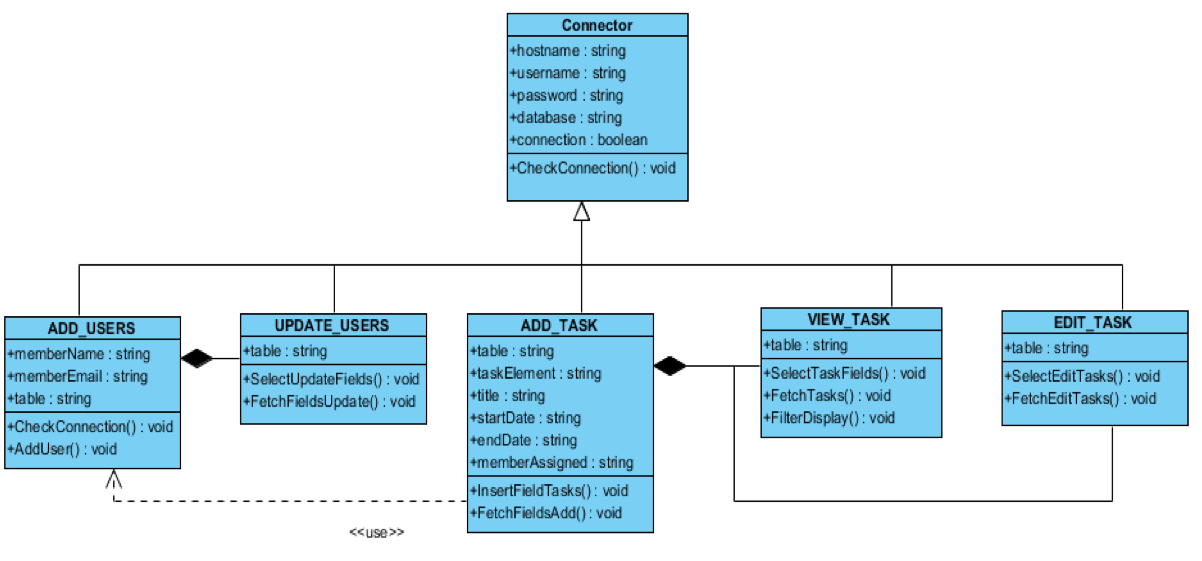
\includegraphics[width=1\textwidth, center]{images/Detailed-Design/TaskerMANClassDiagram} \\
The PHP class diagram above depicts just but a few major collaborating classes in the TaskerMan.  All the classes inherit variables and a single method from the Connector.php.  These variables and the CheckConnection method have to have a constant connection to the database. 
UPDATE\textunderscore USERS class is shown as a composition to the ADD\textunderscore USERS.  This means that it depends solely on the availability of the ADD\textunderscore USERS class.  If the ADD\textunderscore USERS class is removed then UPDATE\textunderscore USERS class will also not exist.
The ADD\textunderscore TASK class is show to make use of the ADD\textunderscore USERS class.  This is where we get our users from.  The VIEW\textunderscore TASK and EDIT\textunderscore TASK   classes are shown as a composition to ADD\textunderscore TASK.

\subsubsection{Description of each significant Class}
\begin{itemize}
\item \textbf{Adding a Task} \\~\\
One file used for processing data is the addtask.php file. This file firstly allows the user to enter in some information such as the start date of the task, completion date and member assigned. Then the information that is typed in, is processed using another PHP file which inserts what the user has typed in to the database, the file firstly connects to the database, checks the connection and then gets all the data the user typed in and adds it to the database. An if statement is then included to check that the data has been entered into the database correctly, if it has, the web page will display a message to the user confirming that a new task has been added to the database, then the user is presented with 3 options to add another task, log out or go back to the home page. If the data is not added to the database correctly due to a problem an error message will be printed out to the user and they won't be able to go on any further in the process. \\~\\
\item \textbf{Edit Tasks} \\~\\
The edittasks.php file presents the user with an area to modify the tasks they have set for example, changing who they have allocated the task to. This connects to the database and prints all of the relevant information in a table - all of the tasks are displayed at this point. From here the user can either update the task or delete the task. If they click on delete, a file called connectedb.php will run and depending on the id that it has (each record in the table has an id for reference purposes) it will then delete all the information from the task list via an SQL command and then closes the database connection. If the user selects the update option from the table they will be taken to a file called updatetask.php this once again is referenced using an ID and once the user clicks this button they are presented with all the information of the task, they can then update the description of the task, change the dates and member allocated.  To get this information, the user is connected to the database and a SELECT SQL query is used. Some text boxes are left open and if the information changes then the field is sent to the database that changes. Once you have updated the records, the user will be able to check their changes have been made by viewing all the tasks. If the update has been successful you will be presented with a confirmation message, if you have not, an error message will be displayed. If you have been successful you will have the option to update another record or go back to the home page. \\~\\
\item \textbf{View Tasks} \\~\\
If you select this option from the home page you will be taken to a file called viewtasks.php. This web page pulls some information from the database using an SQL query to show all of the tasks and then it puts this information into a table to make it easier to read.  This webpage also includes a filter that allows the user to view the data based on the member or the status of the task. Once the user has looked at this information they can either log out or navigate back to the home page. \\~\\
\item \textbf{Add User} \\~\\
If you select the add user option from the home page - you will be presented with two text boxes described earlier in this document. Once you click the submit button you will be taken to a webpage called addusers.php this just adds the information that the user has typed into the database via an SQL command. This once again has an if statement which if unsuccessful will provide the user with a simple error message, if successful in adding the user a confirmation will be shown and then the user will have a few navigation choices. \\~\\
\item \textbf{Edit User} \\~\\
The editusers.php file presents the user with an area to modify their details if they have typed them in wrong or their details change. Currently the only fields we have here are name and email address. If the user wants to update these they just click on the update link and are then taken to an updateusers.php page where they can then re-enter their name and email address. Once they have done that and are happy with it they click the update button which sends the new data they have put in to the database. They will then be provided with a confirmation message if it is successfully updated, and then you can navigate to other areas of the website. To make sure that the user types in information in the correct format we will be implementing some validation to check that the user is entering data of the correct type. Next you can go back to the editusers.php file and also delete records of users. This will be used for managers so that they can delete users from TaskerMAN if they need to. All that they need to do is look at the table of users that is provided in editusers.php and then click on the delete link of the user that they want to get rid of. Once they do that a confirmation message will be displayed telling them that the user has been successfully deleted. Once this action is completed by the user a file called connectdb.php runs which connects to the database and then a delete SQL command is used to get rid of the user they deleted - each user has a reference number, so this is what is used to delete a specific user. Next time they view the edit user's web page the table will have been updated to show all the users they want. To make sure users aren't accidentally deleted we should implement a pop up box to appear and make the user confirm that they want to delete a specific user.  \\~\\
\item \textbf{View Users} \\~\\
Once logged in, view users will enable you to look at all the people using the system - this tool will be used for managers only so they can view all the team members they can allocate tasks too. Once they have clicked on the view user's page, a table will be displayed - this will be populated with information about the users in the system (which will just be their name and email) and what tasks they have been allocated to do. To get this information, an SQL query will be used to select all the users and then this information is just output into a table. 
\end{itemize}
\clearpage
\section{Detailed Design}
\subsection{TaskerSRV Entity-Relationship Diagram}
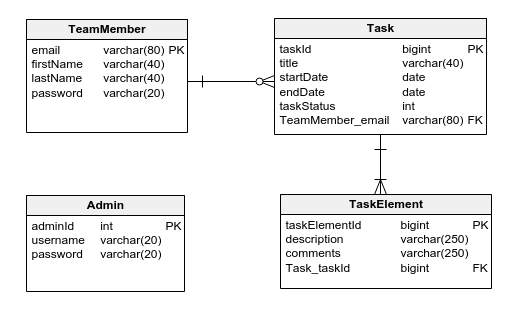
\includegraphics[width=1\textwidth, center]{images/Detailed-Design/taskerSRV} 

\subsection{TaskerCLI Sequence Diagrams}
The following are the sequence diagrams describing the major actions taken by TaskerCLI, namly logging in to the system, updating
a task, logging out, and the synchroniser syncing the changes made to the local and remote databases.

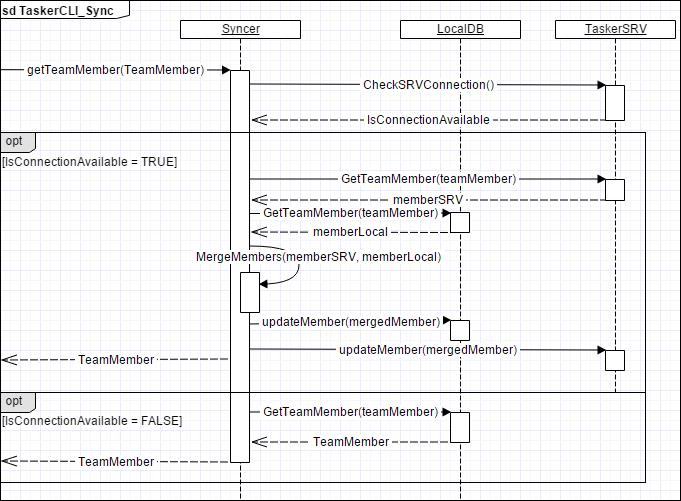
\includegraphics[width=1\textwidth, center]{images/Detailed-Design/TaskerCLISequenceSync} 

Above shows the sequence diagram for the action of syncing the two databases. It works by first checking if TaskerSRV can be connected to,
then branches depending on the connections availability.
If the connection is available, the syncer class gets a copy of the team member from both the local database, and TaskerSRV. It performs
a sort of merge on the two copies, updating information depending on the priority of changes made, clarified in FR9 of the specification document.
It copies this newly merged teamMember object back to both databases, then returns it.

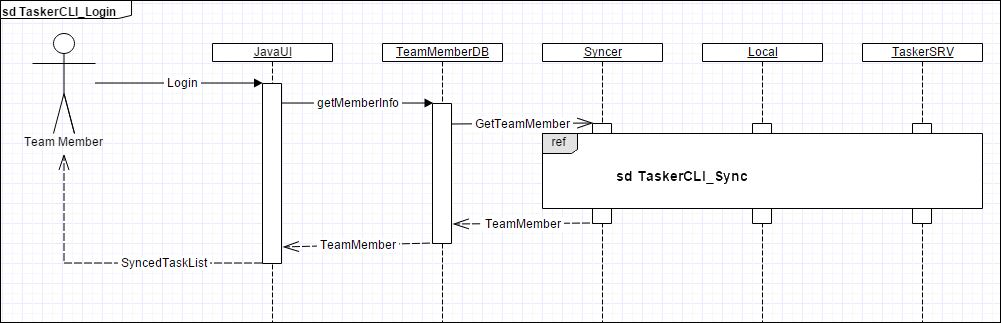
\includegraphics[width=1\textwidth, center]{images/Detailed-Design/TaskerCLISequenceDiagramLogin} 

The above sequence diagram describes the action of a user logging in. The user provides their login details, which the UI sends to
the TeamMemberDB static class. This class sends a request to the Syncer to receive the merged teamMember from both databases.
The syncer runs the actions described in sd TaskerCLI\textunderscore Sync and returns the teamMember to TeamMemberDB, which passes it on to the
UI. The UI pulls the task list from the teamMember, and displays it in the UI for the user.

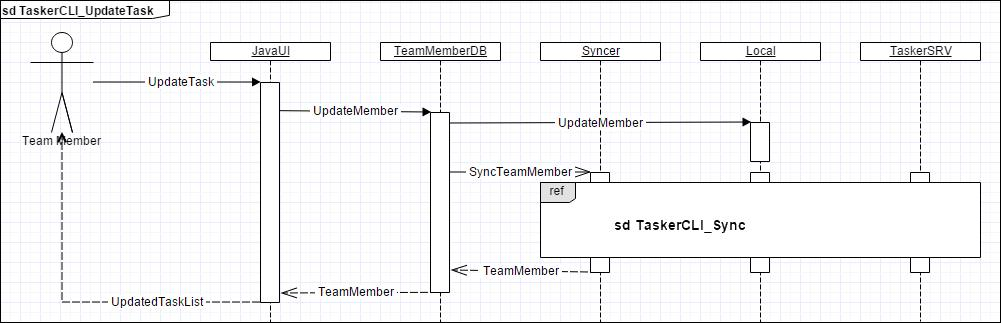
\includegraphics[width=1\textwidth, center]{images/Detailed-Design/TaskerCLISequenceDiagramUpdateTask} 

Above describes what happens when a user updates a task, either by completing it or updating the list of subTasks assigned to it.
The UI sends an update to TeamMemberDB, which first updates the local database with the newly updated task. It then calls on the Syncer
to sync the databases again, using sd TaskerCLI\textunderscore Sync. Because of the priority, the changes made locally will override TaskerSRV if it is available.
The syncer then returns the synced teamMember to TeamMemberDB, which passes it on to the UI. The UI then, like when logging in,
pulls the task list from the teamMember and displays it to the user.

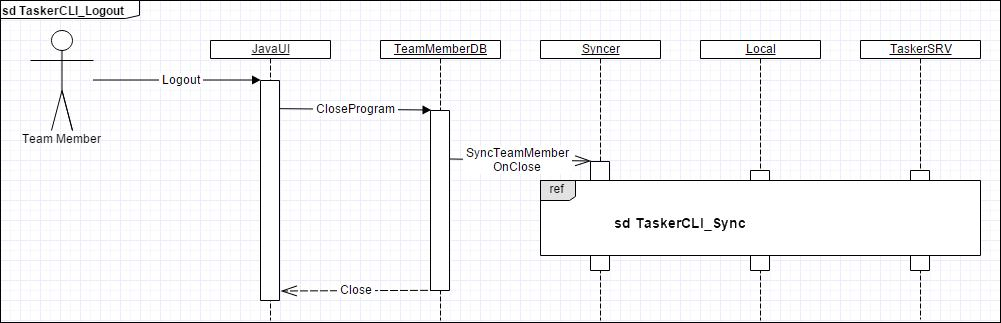
\includegraphics[width=1\textwidth, center]{images/Detailed-Design/TaskerCLISequenceDiagramLogout}

Above describes how TaskerCLI goes about closing when the user logs out. When the user logs out, the UI sends a close command to TeamMemberDB,
telling it to perform a sync with the databases in order to save any last changes before shutting TaskerCLI. It requests a sync from the Syncer,
which synchronises both databases. TeamMemberDB does not request the teamMember be returned as it is not needed. Instead, once the Sync process
is completed, TeamMemberDb sends a message to the UI, telling it that it is ready to shut down. The UI then closes. 

\clearpage

\subsection{Spike Programming} To be able to explore potential solutions to the implementation for Tasker we have created a spike solution by creating a prototype model for both TaskerCLI and TaskerMAN. The spike prototype for TaskerMAN was used in order to experiment running MySQL queries to the database using PHP and also to experiment keeping sessions for the user of the system. The spike prototype for CLI was used to decrease the threat of it being too technically difficult when it came to the actual implementation of TaskerCLI for example, a quickly made spike solution will help us understand how we will structure our classes and relationships between the classes. Our quick spike solutions did not fully support the functional requirements but helped us understand how we can achieve these by giving us an insight on how to structure the more complex areas of the design.   \\
\subsection{TaskerMAN Sequence Diagram}
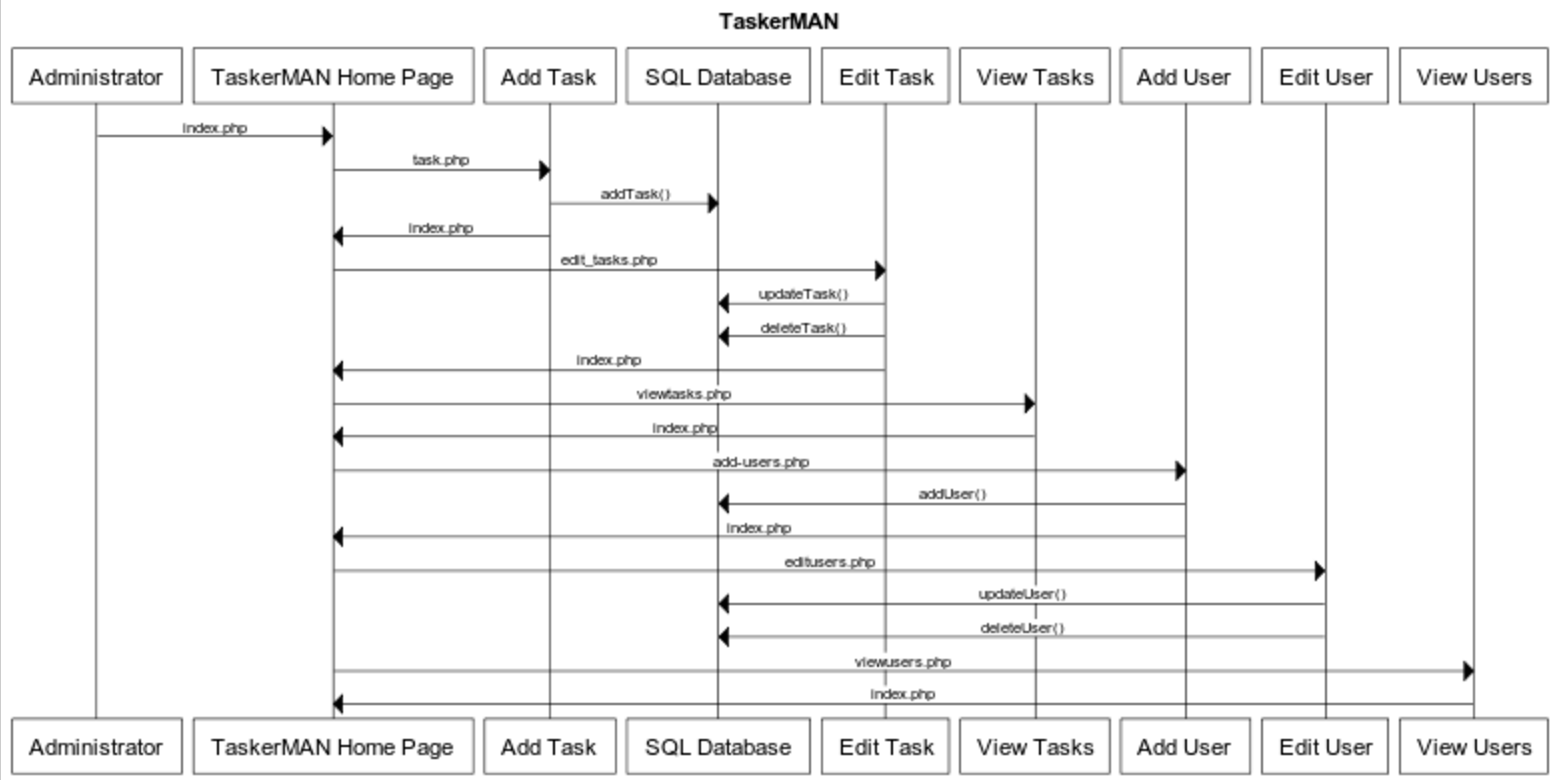
\includegraphics[width=1\textwidth, center]{images/Detailed-Design/TaskerMANSequenceDiagram} \\
\clearpage
\subsection{TaskerMAN Object Diagrams}
\subsubsection{TaskerMAN Object Relationship between the ADD\textunderscore USERS and EDIT\textunderscore USERS CLASS}
Below is an example of the object instances and association in the TaskerMAN at a particular point in time. In this case an instance is created with the user and email of a new member. The two other instances updateMary and DeleteMary are both possible  as a result of the Mary instance in the Add\textunderscore Users class. An example is the diagram showing a wrong spelling name entered in the Mary Instance.  Since the Add\textunderscore Users class has an association with the Edit\textunderscore Users class we can instantiate the UpdateMary instance and correct the name to Mary Joseph. Similarly we can instantiate the DeleteMary instance and delete the member with the wrong name if we wish to. \\
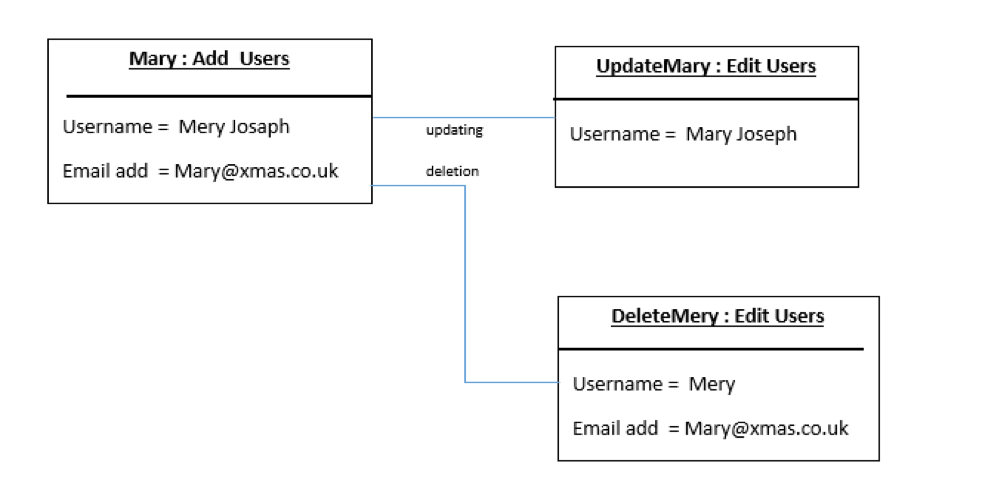
\includegraphics[width=1\textwidth, center]{images/Detailed-Design/TaskerMANObjectDiagram1} \\
\subsubsection{TaskerMAN Object Relationship between the ADD\textunderscore TASK and EDIT\textunderscore TASKS CLASS}
The logic of the object interaction below is essential the same as in above. Here the Mary instance is established and its values are clearly depicted.  All the values in MaryBirth object are correct except the EndDate.  We therefore instantiate the MaryEdit object and make the necessary changes as shown. We can instantiate another object MaryFilter and view the task. \\
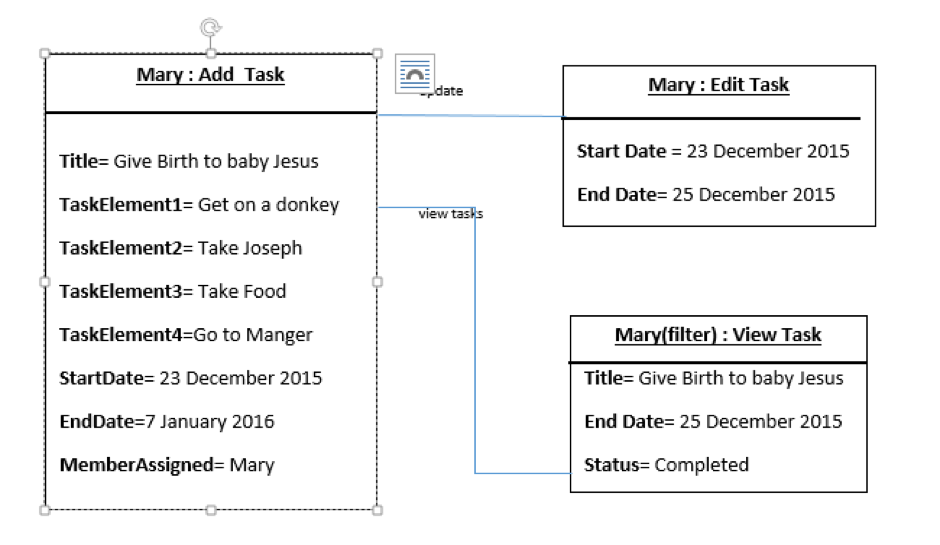
\includegraphics[width=1\textwidth, center]{images/Detailed-Design/TaskerMANObjectDiagram2} \\
\addcontentsline{toc}{section}{REFERENCES}
\begin{thebibliography}{12}
\bibitem{se.qa.ds} \emph{Software Engineering Group Projects}
Design Specification Standards.
C. J. Price, N.W.Hardy and B.P.Tiddeman, SE.QA.05A. 1.8 Release.
\bibitem{se.qa.rs} \emph{Software Engineering Group Projects}
Requirements Specifications.
N. W. Hardy, SE.QA.RS, FR10. 1.1 Release.
\end{thebibliography}
\clearpage
\addcontentsline{toc}{section}{DOCUMENT HISTORY}
\section*{DOCUMENT HISTORY}
\begin{tabular}{|l | l | l | p{8cm} |l | }
\hline
Version & CCF No. & Date & Changes made to Document & Changed by \\
\hline
1.0 & N/A & 2015-10-27 & Initial creation for review & L. Jones \\
\hline
1.1 & N/A & 2015-10-28 & Updated the TaskerCLI user interface section & M. Goly \\
\hline
1.2 & N/A & 2015-10-28 & Created sub-subsections for  Use-cases and User-interface design & L. Jones \\
\hline
1.3 & N/A & 2015-10-29 & Added TaskerCLI Use-Case diagram and narrative & L. Jones \\
\hline
1.4 & N/A & 2015-10-29 & Updated version from review to release & L. Jones \\
\hline
1.5 & N/A & 2015-11-24 & Added Sections for Design Specification Review & L. Jones \\
\hline
1.6 & N/A & 2015-11-27 & Compiled team's  Component Description, Significant Classes and Detailed Design sections for release & L. Jones \\
\hline
1.7 & N/A & 2015-11-27 & Added TaskerSRV diagram and updated the TaskerCLI sequence diagram narrative for release & M. Goly \\
\hline
1.8 & N/A & 2016-02-14 & Updated Java significant classes based on implementation changes for release & J. Mir \\
\hline
\end{tabular}
\label{thelastpage}
\end{document}
\end{verbatim}
\label{fig:footer}
\end{figure}
\label{thelastpage}
\end{document}